\section*{Problems}\addcontentsline{toc}{section}{Problems}
\subsection{Problem 5.4: Positronium lifetime}
\cite{sen2019two}を簡略化した.

\subsubsection{対消滅の不変振幅(0次)}
$e^-e^+ \to 2\gamma$の過程を考える.

\begin{center}
  \feynmandiagram [horizontal=a to b, baseline=(a.base)] {
  i1 [particle=$e^-$] -- [fermion, edge label=$p_1$] a -- [photon, momentum'=$k_1$] i2,
  a -- [fermion, edge label'=$p_1-k_1$] b,
  f2 -- [photon, reversed momentum'=$k_2$] b -- [fermion, reversed momentum=$p_2$] f1 [particle=$e^+$]
  };
  \hfil
  $+$
  \hfil
  \begin{tikzpicture}[arrowlabel/.style={/tikzfeynman/momentum/.cd, arrow shorten=0.37, arrow distance=1.5mm}, arrowlabel/.default=0.4, baseline=(a.base)]
    \begin{feynman}
      \vertex (a);
      \vertex [right=of a] (b);
      \vertex [below left=of a] (i1) {$e^-$};
      \vertex [above left=of a] (f1);
      \vertex [below right=of b] (i2) {$e^+$};
      \vertex [above right=of b] (f2);
      \diagram* {
      (i1) -- [fermion, edge label=$p_1$] (a), (i2) -- [anti fermion, momentum'=$p_2$] (b),
      (a) -- [fermion, edge label'=$p_1-k_2$] (b),
      (a) -- [photon, momentum={[arrowlabel]}, edge label=$k_2$, near end] (f2), (b) -- [photon, momentum'={[arrowlabel]}, edge label'=$k_1$, near end] (f1)
      };
    \end{feynman}
  \end{tikzpicture}
\end{center}

対消滅の不変振幅を運動量$p$の$0$次までの精度で求める.
\begin{align*}
  p_1^\mu  = (E, 0)
  & , &
  p_2^\mu = (E, 0)
  & , &
  k_1^\mu = (E, \boldsymbol{k})
  & , &
  k_2^\mu = (E, -\boldsymbol{k})
  & , &
  \lvert\boldsymbol{k}\rvert = E
  .
\end{align*}
光子の偏極は次のようにおく:
\begin{align*}
  \epsilon_{\pm}^\mu(k_1) = \epsilon_{1\pm}^\mu = (0, \boldsymbol{\epsilon}_1)
  & , &
  \boldsymbol{\epsilon}_1 \cdot \boldsymbol{k}_1 = 0
  & , &
  \epsilon_{\pm}^\mu(k_2) = \epsilon_{2\pm}^\mu = (0, \boldsymbol{\epsilon}_2)
  & , &
  \boldsymbol{\epsilon}_2 \cdot \boldsymbol{k} = 0
  .
\end{align*}
スピノルは次のように近似される:
\begin{align}
  u(p_1) =
  \begin{pmatrix}
    \sqrt{\sigma \cdot p_1} \xi \\
    \sqrt{\overline\sigma \cdot p_1} \xi
  \end{pmatrix}
  \approx \sqrt{m}
  \begin{pmatrix}
    \xi \\
    \xi
  \end{pmatrix}
  & , &
  v(p_2) =
  \begin{pmatrix}
    \sqrt{\sigma \cdot p_2} \eta \\
    -\sqrt{\overline\sigma \cdot p_2} \eta
  \end{pmatrix}
  \approx \sqrt{m}
  \begin{pmatrix}
    \eta \\
    - \eta
  \end{pmatrix}
  . \label{prob5_4a_spinor_approx}
\end{align}
さらに,
\begin{align*}
  p_1 \cdot k_1 = E^2 \approx m^2
  & , &
  p_1 \cdot k_2 = E^2 \approx m^2
  & , &
  (p_1 \cdot k_1)(p_1 \cdot k_2) \approx m^4 .
\end{align*}

Dirac方程式から次を得る:
\begin{align*}
  (\slashed{p}_1 + m) \slashed{\epsilon}_1^\ast u(p_1) &= 2 (p_1 \cdot \epsilon_1^\ast) u(p_1) - \slashed{\epsilon}_1^\ast (\slashed{p}_1 - m) u(p_1) =0 , \\
  (\slashed{p}_1 + m) \slashed{\epsilon}_2^\ast u(p_1) &= 2 (p_1 \cdot \epsilon_2^\ast) u(p_1) - \slashed{\epsilon}_2^\ast (\slashed{p}_1 - m) u(p_1) = 0 .
\end{align*}
従って,不変振幅は
\begin{align}
  \begin{split}
    i\mathcal{M} &= -ie^2 \overline{v}(p_2) \left[ \slashed{\epsilon}_2^\ast \frac{\slashed{p}_1 - \slashed{k}_1 + m}{(p_1 - k_1)^2 - m^2} \slashed{\epsilon}_1^\ast
    + \slashed{\epsilon}_1^\ast \frac{\slashed{p}_1 - \slashed{k}_2 + m}{(p_1 - k_2)^2 - m^2} \slashed{\epsilon}_2^\ast \right] u(p_1) \\
    %
    &= -ie^2 \overline{v}(p_2) \left[ \slashed{\epsilon}_2^\ast \frac{-\slashed{p}_1 + \slashed{k}_1 - m}{2p_1 \cdot k_1} \slashed{\epsilon}_1^\ast
    + \slashed{\epsilon}_1^\ast \frac{-\slashed{p}_1 + \slashed{k}_2 - m}{2p_1 \cdot k_2} \slashed{\epsilon}_2^\ast \right] u(p_1) \\
    %
    &= -i\frac{e^2}{2} \overline{v}(p_2) \left[
    \frac{\slashed{\epsilon}_2^\ast\slashed{k}_1\slashed{\epsilon}_1^\ast}{m^2}
    + \frac{\slashed{\epsilon}_1^\ast\slashed{k}_2\slashed{\epsilon}_2^\ast}{m^2}
    \right] u(p_1) \\
    %
    &= -i\frac{e^2}{2m^2} \overline{v}(p_2) \left[
    \slashed{\epsilon}_2^\ast\slashed{k}_1\slashed{\epsilon}_1^\ast +\slashed{\epsilon}_1^\ast\slashed{k}_2\slashed{\epsilon}_2^\ast
    \right] u(p_1)
  \end{split}
  \label{prob5_4a_iM}
\end{align}
となる.$[\cdots]$を計算するが,まず次の式を示しておく:
\begin{align*}
  \slashed{a}\slashed{b}\slashed{c} &= a_\mu b_\nu c_\rho
  \begin{pmatrix}
    0 & \sigma^\mu \\
    \overline{\sigma}^\mu & 0
  \end{pmatrix}
  \begin{pmatrix}
    0 & \sigma^\nu \\
    \overline{\sigma}^\nu & 0
  \end{pmatrix}
  \begin{pmatrix}
    0 & \sigma^\rho \\
    \overline{\sigma}^\rho & 0
  \end{pmatrix}
  \\
  &= a_\mu b_\nu c_\rho
  \begin{pmatrix}
    0 & \sigma^\mu \overline{\sigma}^\nu \sigma^\rho \\
    \overline{\sigma}^\mu \sigma^\nu \overline{\sigma}^\rho & 0
  \end{pmatrix}
  \\
  &=
  \begin{pmatrix}
    0 & (a \cdot \sigma)(b \cdot \overline\sigma)(c \cdot \sigma) \\
    (a \cdot \overline\sigma)(b \cdot \sigma)(c \cdot \overline\sigma) & 0
  \end{pmatrix}
  .
\end{align*}

\eqref{prob5_4a_iM}の$[\cdots]$のうち3つのガンマ行列を含む項は
\begin{align*}
  \left[ \slashed{\epsilon}_2^\ast\slashed{k}_1\slashed{\epsilon}_1^\ast + \slashed{\epsilon}_1^\ast\slashed{k}_2\slashed{\epsilon}_2^\ast \right]
  & =
  \begin{pmatrix}
    0 & (\epsilon_2^\ast \cdot \sigma)(k_1 \cdot \overline\sigma)(\epsilon_1^\ast \cdot \sigma) \\
    (\epsilon_2^\ast \cdot \overline\sigma)(k_1 \cdot \sigma)(\epsilon_1^\ast \cdot \overline\sigma) & 0
  \end{pmatrix}
  \\
  & +
  \begin{pmatrix}
    0 & (\epsilon_1^\ast \cdot \sigma)(k_2 \cdot \overline\sigma)(\epsilon_2^\ast \cdot \sigma) \\
    (\epsilon_1^\ast \cdot \overline\sigma)(k_2 \cdot \sigma)(\epsilon_2^\ast \cdot \overline\sigma) & 0
  \end{pmatrix}
  \\
  &=
  \begin{pmatrix}
    0 & (\boldsymbol{\epsilon}_2^\ast \cdot \boldsymbol\sigma)(k_1 \cdot \overline\sigma)(\boldsymbol{\epsilon}_1^\ast \cdot \boldsymbol\sigma) \\
    (\boldsymbol{\epsilon}_2^\ast \cdot \boldsymbol\sigma)(k_1 \cdot \sigma)(\boldsymbol{\epsilon}_1^\ast \cdot \boldsymbol\sigma) & 0
  \end{pmatrix}
  \\
  & +
  \begin{pmatrix}
    0 & (\boldsymbol{\epsilon}_1^\ast \cdot \boldsymbol\sigma)(k_2 \cdot \overline\sigma)(\boldsymbol{\epsilon}_2^\ast \cdot \boldsymbol\sigma) \\
    (\boldsymbol{\epsilon}_1^\ast \cdot \boldsymbol\sigma)(k_2 \cdot \sigma)(\boldsymbol{\epsilon}_2^\ast \cdot \boldsymbol\sigma) & 0
  \end{pmatrix}
  \\
  &=:
  \begin{pmatrix}
    0 & m^2\overline{B}_+ \\
    m^2 B_+ & 0
  \end{pmatrix}
  .
\end{align*}

以上から
\begin{align}
  i\mathcal{M}= -i\frac{e^2}{2m^4} \overline{v}(p_2)
  \begin{pmatrix}
    0 & -2m^2A + m^2\overline{B}_+ - (\boldsymbol{p}\cdot\boldsymbol{k}) \overline{B}_- \\
    2m^2A + m^2B_+ - (\boldsymbol{p}\cdot\boldsymbol{k}) B_- & 0
  \end{pmatrix}
  u(p_1) \label{prob5_4a_iM_AB}
\end{align}
となる.各項の定義は
\begin{align}
  \begin{split}
    B_+ &= (\boldsymbol{\epsilon}_1^\ast \cdot \boldsymbol\sigma)(k_2 \cdot \sigma)(\boldsymbol{\epsilon}_2^\ast \cdot \boldsymbol\sigma)
    + (\boldsymbol{\epsilon}_2^\ast \cdot \boldsymbol\sigma)(k_1 \cdot \sigma)(\boldsymbol{\epsilon}_1^\ast \cdot \boldsymbol\sigma) \\
    \overline{B}_+ &= (\boldsymbol{\epsilon}_1^\ast \cdot \boldsymbol\sigma)(k_2 \cdot \overline\sigma)(\boldsymbol{\epsilon}_2^\ast \cdot \boldsymbol\sigma)
    + (\boldsymbol{\epsilon}_2^\ast \cdot \boldsymbol\sigma)(k_1 \cdot \overline\sigma)(\boldsymbol{\epsilon}_1^\ast \cdot \boldsymbol\sigma)
    .
  \end{split}
  \label{prob5_4a_AB_def}
\end{align}

$(\boldsymbol\sigma \cdot \boldsymbol{a}) (\boldsymbol\sigma \cdot \boldsymbol{b}) = \boldsymbol{a} \cdot \boldsymbol{b} + i \boldsymbol\sigma \cdot (\boldsymbol{a} \times \boldsymbol{b})$から
\begin{align*}
  (\boldsymbol{\epsilon}_1^\ast \cdot \boldsymbol\sigma)(\boldsymbol{k}\cdot\boldsymbol\sigma)(\boldsymbol{\epsilon}_2^\ast \cdot \boldsymbol\sigma)
  &= [\boldsymbol{\epsilon}_1^\ast \cdot \boldsymbol{k} + i \boldsymbol\sigma \cdot (\boldsymbol{\epsilon}_1^\ast \times \boldsymbol{k})](\boldsymbol{\epsilon}_2^\ast \cdot \boldsymbol\sigma) \\
  &= i \boldsymbol\sigma \cdot (\boldsymbol{\epsilon}_1^\ast \times \boldsymbol{k})(\boldsymbol{\epsilon}_2^\ast \cdot \boldsymbol\sigma) \\
  &= i (\boldsymbol{\epsilon}_1^\ast \times \boldsymbol{k}) \cdot \boldsymbol{\epsilon}_2^\ast - \boldsymbol\sigma \cdot [(\boldsymbol{\epsilon}_1^\ast \times \boldsymbol{k}) \times \boldsymbol{\epsilon}_2^\ast] \\
  &= i (\boldsymbol{\epsilon}_2^\ast \times \boldsymbol{\epsilon}_1^\ast) \cdot \boldsymbol{k} - \boldsymbol\sigma \cdot [(\boldsymbol{\epsilon}_1^\ast \cdot \boldsymbol{\epsilon}_2^\ast) \boldsymbol{k} - (\boldsymbol{k} \cdot \boldsymbol{\epsilon}_2^\ast) \boldsymbol{\epsilon}_1^\ast] \\
  &= - i (\boldsymbol{\epsilon}_1^\ast \times \boldsymbol{\epsilon}_2^\ast) \cdot \boldsymbol{k}
  - (\boldsymbol\sigma \cdot \boldsymbol{k})(\boldsymbol{\epsilon}_1^\ast \cdot \boldsymbol{\epsilon}_2^\ast) \\
  %
  (\boldsymbol{\epsilon}_2^\ast \cdot \boldsymbol\sigma)(\boldsymbol{k}\cdot\boldsymbol\sigma)(\boldsymbol{\epsilon}_1^\ast \cdot \boldsymbol\sigma)
  &=  i (\boldsymbol{\epsilon}_1^\ast \times \boldsymbol{\epsilon}_2^\ast) \cdot \boldsymbol{k}
  - (\boldsymbol\sigma \cdot \boldsymbol{k})(\boldsymbol{\epsilon}_1^\ast \cdot \boldsymbol{\epsilon}_2^\ast) \\
\end{align*}
となる.従って,
\begin{align}
  \begin{split}
    \overline{B}_+ - B_+ &= (\boldsymbol{\epsilon}_1^\ast \cdot \boldsymbol\sigma)(k_2 \cdot \overline\sigma)(\boldsymbol{\epsilon}_2^\ast \cdot \boldsymbol\sigma)
    + (\boldsymbol{\epsilon}_2^\ast \cdot \boldsymbol\sigma)(k_1 \cdot \overline\sigma)(\boldsymbol{\epsilon}_1^\ast \cdot \boldsymbol\sigma) \\
    &- (\boldsymbol{\epsilon}_1^\ast \cdot \boldsymbol\sigma)(k_2 \cdot \sigma)(\boldsymbol{\epsilon}_2^\ast \cdot \boldsymbol\sigma)
    - (\boldsymbol{\epsilon}_2^\ast \cdot \boldsymbol\sigma)(k_1 \cdot \sigma)(\boldsymbol{\epsilon}_1^\ast \cdot \boldsymbol\sigma) \\
    &= (\boldsymbol{\epsilon}_1^\ast \cdot \boldsymbol\sigma)(k_2 \cdot (\overline\sigma - \sigma))(\boldsymbol{\epsilon}_2^\ast \cdot \boldsymbol\sigma)
    + (\boldsymbol{\epsilon}_2^\ast \cdot \boldsymbol\sigma)(k_1 \cdot (\overline\sigma - \sigma))(\boldsymbol{\epsilon}_1^\ast \cdot \boldsymbol\sigma) \\
    &= -2(\boldsymbol{\epsilon}_1^\ast \cdot \boldsymbol\sigma)(\boldsymbol{k}\cdot\boldsymbol\sigma)(\boldsymbol{\epsilon}_2^\ast \cdot \boldsymbol\sigma)
    + 2(\boldsymbol{\epsilon}_2^\ast \cdot \boldsymbol\sigma)(\boldsymbol{k}\cdot\boldsymbol\sigma)(\boldsymbol{\epsilon}_1^\ast \cdot \boldsymbol\sigma) \\
    &= 4i (\boldsymbol{\epsilon}_1^\ast \times \boldsymbol{\epsilon}_2^\ast) \cdot \boldsymbol{k} , \\
  \end{split}
  \label{prob5_4a_BBB}
\end{align}

\eqref{prob5_4a_iM_AB}に\eqref{prob5_4a_spinor_approx}を代入して,\eqref{prob5_4a_BBB}を使えば,
\begin{align}
  \begin{split}
    i\mathcal{M}(e^-_se^+_r \to 2\gamma) &= -i\frac{e^2}{2m^2} \overline{v}(p_2)
    \begin{pmatrix}
      0 & \overline{B}_+ \\
      B_+ & 0
    \end{pmatrix}
    u(p_1) \\
    %
    &= -i\frac{e^2}{2m}
    \begin{pmatrix}
      \eta^{r\dagger} & - \eta^{r\dagger}
    \end{pmatrix}
    \begin{pmatrix}
      0 & 1 \\
      1 & 0
    \end{pmatrix}
    \begin{pmatrix}
      0 & \overline{B}_+ \\
      B_+ & 0
    \end{pmatrix}
    \begin{pmatrix}
      \xi^s \\
      \xi^s
    \end{pmatrix}
    \\
    %
    &= i\frac{e^2}{2m} \eta^{r\dagger} (\overline{B}_+ - B_+) \xi^s \\
    %
    &= - \frac{2e^2}{m} (\boldsymbol{\epsilon}_1^\ast \times \boldsymbol{\epsilon}_2^\ast) \cdot \boldsymbol{k} (\eta^{r\dagger} \xi^s)
  \end{split}
  \label{prob5_4a_iM_cal}
\end{align}
となる.

ここで,各スピノルは(3.135)(3.136)から
\begin{align}
  \xi^\uparrow =
  \begin{pmatrix}
    1 \\
    0
  \end{pmatrix}
  &, &
  \xi^\downarrow =
  \begin{pmatrix}
    0 \\
    1
  \end{pmatrix}
  &, &
  \eta^\uparrow =
  \begin{pmatrix}
    0 \\
    1
  \end{pmatrix}
  &, &
  \eta^\downarrow =
  \begin{pmatrix}
    -1 \\
    0
  \end{pmatrix}
  \label{prob5_4a_spinor}
\end{align}
で与えられる.ラベルは全て電子・陽電子のスピンを表す.
% 電子と陽電子は逆向きに動くので,spinが逆ならhelicityは一致する.

\subsubsection{Sポジトロニウムの構成}
束縛状態の式(5.43)
\[ \ket{B} = \sqrt{2M} \int \frac{d^3k}{(2\pi)^3} \tilde\psi(\boldsymbol{k}) \frac{1}{\sqrt{2m}} \frac{1}{\sqrt{2m}} \ket{\boldsymbol{k}\uparrow, -\boldsymbol{k}\uparrow} \]
を角運動量を考慮した形に拡張する.
すなわち,スピン$S$,軌道角運動量$l$,全角運動量$J$,全角運動量の射影$M$の状態$\ket{^{2S+1}l_J; M}$を構成しよう
\footnote{スピンは粒子の内在的な量なので,電子のスピン,陽電子のスピンを足す.それに対し軌道角運動量は粒子の相対運動に起因するので,電子と陽電子について和を取ることは行わない}.
これには,スピンの射影が$S_z$で軌道角運動量の射影が$M-S_Z=:m$の状態をClebash-Gordan係数$\braket{lS; mS_z | lS; JM}$によって足せば良い:
\begin{align}
  \ket{^{2S+1}l_J; M} = \sqrt{2M} \int \frac{d^3p}{(2\pi)^3} \sum_{S_z=-S}^S
  \braket{lS; mS_z | lS; JM} \tilde{\psi}_{lm}(\boldsymbol{p}) \ket{S, S_z}_{\boldsymbol{p}}
  \label{prob5_4a_Ps_wf}
\end{align}
(ただし,慣例に従い$l=0$は$S$,$l=1$は$P$などと表記する).
なお,電子の運動量は$\boldsymbol{p}$,陽電子の運動量は$-\boldsymbol{p}$とする.
換算質量は$m/2$なので,相対運動量は$\boldsymbol{p}$である.

\begin{center}
  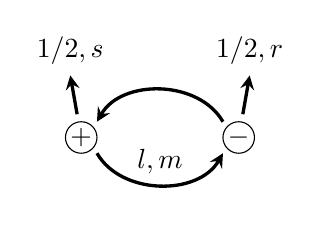
\begin{tikzpicture}[>=stealth]
    \draw (0, 0) circle [radius=0.2] node {$+$};
    \draw[very thick, ->] (100: 0.3) -- (100: 0.8) node [above] {$1/2, s$};
    \begin{scope}[xshift=2cm]
      \draw (0, 0) circle [radius=0.2] node {$-$};
      \draw[very thick, ->] (80: 0.3) -- (80: 0.8) node [above] {$1/2, r$};
    \end{scope}
    \draw[very thick, ->] (0.2, -0.2) to [out=-60, in =-120] (1.8, -0.2);
    \draw[very thick, ->] (1.8, 0.2) to [out=120, in =60] (0.2, 0.2);
    \draw (1, -0.3) node {$l, m$};
  \end{tikzpicture}
\end{center}

(電子と陽電子の合計)スピン$S$,射影$S_z$,相対運動量$\boldsymbol{p}$の状態$\ket{S, S_z}_{\boldsymbol{p}}$は,
スピン射影$s$で運動量$\boldsymbol{p}$の電子と,スピン射影$r:=S_z-s$で運動量$\boldsymbol{p}$の陽電子の線形結合で表せる:
\begin{align*}
  \ket{S, S_z}_{\boldsymbol{p}} &= \sum_s \Braket{ \frac{1}{2} \frac{1}{2}; s r | \frac{1}{2} \frac{1}{2}; S S_z} \Ket{\frac{1}{2}, s}_{\boldsymbol{p}} \Ket{\frac{1}{2}, r}_{-\boldsymbol{p}} \\
  &= \sum_s \Braket{ \frac{1}{2} \frac{1}{2}; s r | \frac{1}{2} \frac{1}{2}; S S_z}
  \frac{1}{\sqrt{2m}} \frac{1}{\sqrt{2m}} a_{\boldsymbol{p}}^{s\dagger} b_{-\boldsymbol{p}}^{r\dagger} \ket{0} .
\end{align*}

まず,$S$状態($l=0$)のポジトロニウムについて考える($m=0$なので$M=S_z$).
$\ket{^1S_0; 0}$は$J=M=0$, $S=S_z=0$なのでスピンはsinglet:
\begin{align}
  \ket{^1S_0; 0} = 2\sqrt{m} \int \frac{d^3p}{(2\pi)^3} \tilde{\psi}_{00}(\boldsymbol{p}) \frac{1}{\sqrt{2m}} \frac{1}{\sqrt{2m}}
  \frac{\ket{\boldsymbol{p} \uparrow, -\boldsymbol{p} \downarrow} - \ket{\boldsymbol{p} \downarrow, -\boldsymbol{p} \uparrow}}{\sqrt{2}} .
  \label{prob5_4a_1S_0;0}
\end{align}
$\ket{^3S_1; 0}$は$J=1$, $M=0$, $S=1$, $S_z=0$なのでスピンはtriplet:
\begin{align*}
  \ket{^3S_1; 0} = 2\sqrt{m} \int \frac{d^3p}{(2\pi)^3} \tilde{\psi}_{00}(\boldsymbol{p}) \frac{1}{\sqrt{2m}} \frac{1}{\sqrt{2m}}
  \frac{\ket{\boldsymbol{p} \uparrow, -\boldsymbol{p} \downarrow} + \ket{\boldsymbol{p} \downarrow, -\boldsymbol{p} \uparrow}}{\sqrt{2}} .
\end{align*}
$\ket{^3S_1; 1}$は$J=1$, $M=1$, $S=1$, $S_z=1$なのでスピンはtriplet:
\begin{align*}
  \ket{^3S_1; 1} = 2\sqrt{m} \int \frac{d^3p}{(2\pi)^3} \tilde{\psi}_{00}(\boldsymbol{p}) \frac{1}{\sqrt{2m}} \frac{1}{\sqrt{2m}} \ket{\boldsymbol{p} \uparrow, -\boldsymbol{p} \uparrow} .
\end{align*}
$\ket{^3S_1; -1}$は$J=1$, $M=-1$, $S=1$, $S_z=-1$なのでスピンはtriplet:
\begin{align*}
  \ket{^3S_1; -1} = 2\sqrt{m} \int \frac{d^3p}{(2\pi)^3} \tilde{\psi}_{00}(\boldsymbol{p}) \frac{1}{\sqrt{2m}} \frac{1}{\sqrt{2m}} \ket{\boldsymbol{p} \downarrow, -\boldsymbol{p} \downarrow} .
\end{align*}

\subsubsection{Sポジトロニウムの崩壊}
不変振幅$\mathcal{M}$の定義(4.73)に注意して,\eqref{prob5_4a_iM_cal}\eqref{prob5_4a_spinor}\eqref{prob5_4a_1S_0;0}から
\begin{align}
  \begin{split}
    i\mathcal{M}(^1S_0 \to 2\gamma) &= 2\sqrt{m} \int \frac{d^3p}{(2\pi)^3} \tilde{\psi}_{00}(\boldsymbol{p}) \frac{1}{2m}
    \frac{i\mathcal{M}(e^-_\uparrow e^+_\downarrow \to 2\gamma) - i\mathcal{M}(e^-_\downarrow e^+_\uparrow \to 2\gamma)}{\sqrt{2}} \\
    &= 2\sqrt{m} \int \frac{d^3p}{(2\pi)^3} \tilde{\psi}_{00}(\boldsymbol{p}) \frac{1}{2m} \left( -\frac{2e^2}{m} \right) (\boldsymbol{\epsilon}_1^\ast \times \boldsymbol{\epsilon}_2^\ast) \cdot \boldsymbol{k}
    \frac{ \eta^{\downarrow\dagger}\xi^\uparrow - \eta^{\uparrow\dagger}\xi^\downarrow}{\sqrt{2}} \\
    &= 2\sqrt{m} \int \frac{d^3p}{(2\pi)^3} \tilde{\psi}_{00}(\boldsymbol{p}) \frac{1}{2m} \left( -\frac{2e^2}{m} \right) (\boldsymbol{\epsilon}_1^\ast \times \boldsymbol{\epsilon}_2^\ast) \cdot \boldsymbol{k} \frac{-2}{\sqrt{2}} \\
    &= 2\sqrt{m} \int \frac{d^3p}{(2\pi)^3} \tilde{\psi}_{00}(\boldsymbol{p}) \frac{1}{2m} \left( -\frac{2e^2}{m} \right) (\boldsymbol{\epsilon}_1^\ast \times \boldsymbol{\epsilon}_2^\ast) \cdot \boldsymbol{k} \frac{-2}{\sqrt{2}} \\
    &= 2\sqrt{2} \frac{e^2}{m\sqrt{m}}  (\boldsymbol{\epsilon}_1^\ast \times \boldsymbol{\epsilon}_2^\ast) \cdot \boldsymbol{k} \int \frac{d^3p}{(2\pi)^3} \tilde{\psi}_{00}(\boldsymbol{p}) \\
    &= 2\sqrt{2} \frac{e^2}{m\sqrt{m}} (\boldsymbol{\epsilon}_1^\ast \times \boldsymbol{\epsilon}_2^\ast) \cdot \boldsymbol{k} \psi_{00}(0) .
  \end{split}
  \label{prob5_4a_1S_0_2hv}
\end{align}

(A.26)から
\[ \sum_\text{polarization} \epsilon^{\mu\ast}\epsilon^\nu \to -g^{\mu\nu} \]
なので,
\begin{align}
  \begin{split}
    \lvert (\boldsymbol{\epsilon}_1^\ast \times \boldsymbol{\epsilon}_2^\ast) \cdot \boldsymbol{k} \rvert^2
    &= \sum_\text{pol 1}\sum_\text{pol 2}\sum_{ijklmn} \epsilon^{ijk} \epsilon_1^{i\ast}\epsilon_2^{j\ast} k^k \epsilon^{lmn} \epsilon_1^l\epsilon_2^m k^n \\
    &\to \sum_{ijklmn} \epsilon^{ijk}\epsilon^{lmn} g^{il} g^{jm} k^k k^n \\
    &= \sum_{klmn} \epsilon^{lmk}\epsilon^{lmn} k^k k^n \\
    &= \sum_{lmn} \epsilon^{lmn}\epsilon^{lmn} k^n k^n \\
    &= 2\lvert\boldsymbol{k}\rvert^2 = 2E^2 \approx 2m^2
  \end{split}
  \label{prob5_4a_pol_sum}
\end{align}
を得る.

$n=1$の場合\footnote{換算質量は$m/2$なので,Bohr半径$a_0 = 2/\alpha m$}を考える.
\[ \psi_{100} = R_{10}(r) Y_{00}(\theta, \phi) = \frac{1}{\sqrt{4\pi}} \frac{2}{a_0{}^{3/2}} \exp \left( - \frac{r}{2a_0} \right) \]
なので,
\begin{align}
  \lvert \psi_{100}(0) \rvert^2 = \frac{m^3\alpha^3}{8\pi} . \label{prob5_4a_wf_100}
\end{align}
\eqref{prob5_4a_1S_0_2hv}\eqref{prob5_4a_pol_sum}\eqref{prob5_4a_wf_100}から
\begin{align}
  \sum_\text{polarization} \lvert \mathcal{M}(1^1S_0 \to 2\gamma) \rvert^2 &= 8 \frac{e^4}{m^3} 2m^2 \frac{m^3\alpha^3}{8\pi} = 32\pi m^2 \alpha^5 .
\end{align}
(4.86)から
\begin{align*}
  \Gamma(1^1S_0 \to 2\gamma) &= \frac{1}{2} \frac{1}{4m} \int \frac{d^3k_1}{(2\pi)^3}\frac{d^3k_2}{(2\pi)^3} \frac{1}{4E_1E_2} \lvert \mathcal{M}(^1S_0 \to 2\gamma) \rvert^2 (2\pi)^4 \mathop{\delta^{(4)}}(k_1+k_2-p_1-p_2) \\
  &= \frac{1}{8m} \int \frac{d^3k_1}{(2\pi)^2} \frac{1}{4\lvert \boldsymbol{k}_1 \rvert^2} 32\pi m^2 \alpha^5 \mathop\delta(2E_1 - 2m) \\
  &= \pi m\alpha^5 4\pi \int \frac{d\lvert \boldsymbol{k}_1 \rvert}{(2\pi)^2} \frac{1}{2} \mathop\delta(\lvert \boldsymbol{k}_1 \rvert - m) \\
  &= \frac{m\alpha^5}{2}
\end{align*}
(出てくる光子は区別できないので,$1/2$倍する).

\eqref{prob5_4a_1S_0_2hv}と同様に考えれば,
\begin{align*}
  \eta^{\uparrow\dagger}\xi^\uparrow = 0
  & , &
  \frac{\eta^{\uparrow\dagger}\xi^\downarrow + \eta^{\downarrow\dagger}\xi^\uparrow}{\sqrt{2}} = 0
  & , &
  \eta^{\downarrow\dagger}\xi^\downarrow = 0
\end{align*}
なので,$\mathcal{M}(^3S_1 \to 2\gamma) = 0$であることが分かる.
すなわち,スピン$1$の$1^3S$は2光子に崩壊しない.

\subsubsection{対消滅の不変振幅(1次)}
対消滅の不変振幅を運動量$p$の$1$次までの精度で求める.
\begin{align*}
  p_1^\mu  = (E, \boldsymbol{p})
  & , &
  p_2^\mu = (E, -\boldsymbol{p})
  & , &
  k_1^\mu = (E, \boldsymbol{k})
  & , &
  k_2^\mu = (E, -\boldsymbol{k})
  .
\end{align*}
光子の偏極は次のようにおく:
\begin{align*}
  \epsilon_{\pm}^\mu(k_1) = \epsilon_{1\pm}^\mu = (0, \boldsymbol{\epsilon}_1)
  & , &
  \boldsymbol{\epsilon}_1 \cdot \boldsymbol{k}_1 = 0
  & , &
  \epsilon_{\pm}^\mu(k_2) = \epsilon_{2\pm}^\mu = (0, \boldsymbol{\epsilon}_2)
  & , &
  \boldsymbol{\epsilon}_2 \cdot \boldsymbol{k}_2 = 0
  .
\end{align*}
スピノルは次のように近似される:
\begin{align}
  u(p_1) =
  \begin{pmatrix}
    \sqrt{\sigma \cdot p_1} \xi \\
    \sqrt{\overline\sigma \cdot p_1} \xi
  \end{pmatrix}
  \approx \sqrt{m}
  \begin{pmatrix}
    \left( 1 - \dfrac{\boldsymbol\sigma \cdot \boldsymbol{p}}{2m} \right) \xi \\[10pt]
    \left( 1 + \dfrac{\boldsymbol\sigma \cdot \boldsymbol{p}}{2m} \right) \xi
  \end{pmatrix}
  & , &
  v(p_2) =
  \begin{pmatrix}
    \sqrt{\sigma \cdot p_2} \eta \\
    -\sqrt{\overline\sigma \cdot p_2} \eta
  \end{pmatrix}
  \approx \sqrt{m}
  \begin{pmatrix}
    \left( 1 + \dfrac{\boldsymbol\sigma \cdot \boldsymbol{p}}{2m} \right) \eta \\[10pt]
    -\left( 1 - \dfrac{\boldsymbol\sigma \cdot \boldsymbol{p}}{2m} \right) \eta
  \end{pmatrix}
  . \label{prob5_4b_spinor_approx}
\end{align}
さらに,
\begin{align*}
  p_1 \cdot k_1 &= E^2 - \boldsymbol{p} \cdot \boldsymbol{k} \approx m^2 - \boldsymbol{p} \cdot \boldsymbol{k}, \\
  p_1 \cdot k_2 &= E^2 + \boldsymbol{p} \cdot \boldsymbol{k} \approx m^2 + \boldsymbol{p} \cdot \boldsymbol{k}, \\
  (p_1 \cdot k_1)(p_1 \cdot k_2) &\approx m^4 .
\end{align*}

Dirac方程式から次を得る:
\begin{align*}
  (\slashed{p}_1 + m) \slashed{\epsilon}_1^\ast u(p_1) &= 2 (p_1 \cdot \epsilon_1^\ast) u(p_1) - \slashed{\epsilon}_1^\ast (\slashed{p}_1 - m) u(p_1) = 2 (p_1 \cdot \epsilon_1^\ast) u(p_1) , \\
  (\slashed{p}_1 + m) \slashed{\epsilon}_2^\ast u(p_1) &= 2 (p_1 \cdot \epsilon_2^\ast) u(p_1) - \slashed{\epsilon}_2^\ast (\slashed{p}_1 - m) u(p_1) = 2 (p_1 \cdot \epsilon_2^\ast) u(p_1) .
\end{align*}
従って,不変振幅は
\begin{align}
  \begin{split}
    i\mathcal{M} &= -ie^2 \overline{v}(p_2) \left[ \slashed{\epsilon}_2^\ast \frac{\slashed{p}_1 - \slashed{k}_1 + m}{(p_1 - k_1)^2 - m^2} \slashed{\epsilon}_1^\ast
    + \slashed{\epsilon}_1^\ast \frac{\slashed{p}_1 - \slashed{k}_2 + m}{(p_1 - k_2)^2 - m^2} \slashed{\epsilon}_2^\ast \right] u(p_1) \\
    %
    &= -ie^2 \overline{v}(p_2) \left[ \slashed{\epsilon}_2^\ast \frac{-\slashed{p}_1 + \slashed{k}_1 - m}{2p_1 \cdot k_1} \slashed{\epsilon}_1^\ast
    + \slashed{\epsilon}_1^\ast \frac{-\slashed{p}_1 + \slashed{k}_2 - m}{2p_1 \cdot k_2} \slashed{\epsilon}_2^\ast \right] u(p_1) \\
    %
    &= -i\frac{e^2}{2} \overline{v}(p_2) \left[
    \frac{\slashed{\epsilon}_2^\ast\slashed{k}_1\slashed{\epsilon}_1^\ast - 2(p_1 \cdot \epsilon_1^\ast)\slashed{\epsilon}_2^\ast}{m^2 - \boldsymbol{p} \cdot \boldsymbol{k}}
    + \frac{\slashed{\epsilon}_1^\ast\slashed{k}_2\slashed{\epsilon}_2^\ast - 2(p_1 \cdot \epsilon_2^\ast)\slashed{\epsilon}_1^\ast}{m^2 + \boldsymbol{p} \cdot \boldsymbol{k}}
    \right] u(p_1) \\
    %
    &= -i\frac{e^2}{2m^4} \overline{v}(p_2) \left[
    (m^2 + \boldsymbol{p} \cdot \boldsymbol{k})(\slashed{\epsilon}_2^\ast\slashed{k}_1\slashed{\epsilon}_1^\ast - 2(p_1 \cdot \epsilon_1^\ast)\slashed{\epsilon}_2^\ast)
    + (m^2 - \boldsymbol{p} \cdot \boldsymbol{k})(\slashed{\epsilon}_1^\ast\slashed{k}_2\slashed{\epsilon}_2^\ast - 2(p_1 \cdot \epsilon_2^\ast)\slashed{\epsilon}_1^\ast)
    \right] u(p_1)
  \end{split}
  \label{prob5_4b_iM}
\end{align}
となる.$[\cdots]$を計算するが,まず次の式を示しておく:
\begin{align*}
  \slashed{a}\slashed{b}\slashed{c} &= a_\mu b_\nu c_\rho
  \begin{pmatrix}
    0 & \sigma^\mu \\
    \overline{\sigma}^\mu & 0
  \end{pmatrix}
  \begin{pmatrix}
    0 & \sigma^\nu \\
    \overline{\sigma}^\nu & 0
  \end{pmatrix}
  \begin{pmatrix}
    0 & \sigma^\rho \\
    \overline{\sigma}^\rho & 0
  \end{pmatrix}
  \\
  &= a_\mu b_\nu c_\rho
  \begin{pmatrix}
    0 & \sigma^\mu \overline{\sigma}^\nu \sigma^\rho \\
    \overline{\sigma}^\mu \sigma^\nu \overline{\sigma}^\rho & 0
  \end{pmatrix}
  \\
  &=
  \begin{pmatrix}
    0 & (a \cdot \sigma)(b \cdot \overline\sigma)(c \cdot \sigma) \\
    (a \cdot \overline\sigma)(b \cdot \sigma)(c \cdot \overline\sigma) & 0
  \end{pmatrix}
  .
\end{align*}

\eqref{prob5_4b_iM}の$[\cdots]$のうち$m^2$と1つのガンマ行列を含む項は
\begin{align*}
  & -2m^2 (p_1 \cdot \epsilon_1^\ast) \slashed{\epsilon}_2^\ast -2m^2 (p_1 \cdot \epsilon_2^\ast) \slashed{\epsilon}_1^\ast  \\
  &= -2m^2 (p_1 \cdot \epsilon_1^\ast)
  \begin{pmatrix}
    0 & \epsilon_2^\ast \cdot \sigma \\
    \epsilon_2^\ast \cdot \overline\sigma & 0
  \end{pmatrix}
  -2m^2 (p_1 \cdot \epsilon_2^\ast)
  \begin{pmatrix}
    0 & \epsilon_1^\ast \cdot \sigma \\
    \epsilon_1^\ast \cdot \overline\sigma & 0
  \end{pmatrix}
  \\
  %
  &= -2m^2 (\boldsymbol{p} \cdot \boldsymbol{\epsilon}_1^\ast)
  \begin{pmatrix}
    0 & \boldsymbol{\epsilon}_2^\ast \cdot \boldsymbol\sigma \\
    -\boldsymbol{\epsilon}_2^\ast \cdot \boldsymbol\sigma & 0
  \end{pmatrix}
  -2m^2 (\boldsymbol{p} \cdot \boldsymbol{\epsilon}_2^\ast)
  \begin{pmatrix}
    0 & \boldsymbol{\epsilon}_1^\ast \cdot \boldsymbol\sigma \\
    -\boldsymbol{\epsilon}_1^\ast \cdot \boldsymbol\sigma & 0
  \end{pmatrix}
  \\
  %
  &= -2m^2
  \begin{pmatrix}
    0 & (\boldsymbol{p} \cdot \boldsymbol{\epsilon}_1^\ast)(\boldsymbol{\epsilon}_2^\ast \cdot \boldsymbol\sigma)
    + (\boldsymbol{p} \cdot \boldsymbol{\epsilon}_2^\ast)(\boldsymbol{\epsilon}_1^\ast \cdot \boldsymbol\sigma)
    \\
    -(\boldsymbol{p} \cdot \boldsymbol{\epsilon}_1^\ast)(\boldsymbol{\epsilon}_2^\ast \cdot \boldsymbol\sigma)
    - (\boldsymbol{p} \cdot \boldsymbol{\epsilon}_2^\ast)(\boldsymbol{\epsilon}_1^\ast \cdot \boldsymbol\sigma)
    & 0
  \end{pmatrix}
  \\
  & =:
  \begin{pmatrix}
    0 & -2m^2 A \\
    2m^2 A & 0
  \end{pmatrix}
  .
\end{align*}

\eqref{prob5_4b_iM}の$[\cdots]$のうち$m^2$と3つのガンマ行列を含む項は
\begin{align*}
  & m^2\left[ \slashed{\epsilon}_2^\ast\slashed{k}_1\slashed{\epsilon}_1^\ast + \slashed{\epsilon}_1^\ast\slashed{k}_2\slashed{\epsilon}_2^\ast \right] \\
  &\quad = m^2
  \begin{pmatrix}
    0 & (\epsilon_2^\ast \cdot \sigma)(k_1 \cdot \overline\sigma)(\epsilon_1^\ast \cdot \sigma) \\
    (\epsilon_2^\ast \cdot \overline\sigma)(k_1 \cdot \sigma)(\epsilon_1^\ast \cdot \overline\sigma) & 0
  \end{pmatrix}
  \\
  & \quad + m^2
  \begin{pmatrix}
    0 & (\epsilon_1^\ast \cdot \sigma)(k_2 \cdot \overline\sigma)(\epsilon_2^\ast \cdot \sigma) \\
    (\epsilon_1^\ast \cdot \overline\sigma)(k_2 \cdot \sigma)(\epsilon_2^\ast \cdot \overline\sigma) & 0
  \end{pmatrix}
  \\
  &\quad = m^2
  \begin{pmatrix}
    0 & (\boldsymbol{\epsilon}_2^\ast \cdot \boldsymbol\sigma)(k_1 \cdot \overline\sigma)(\boldsymbol{\epsilon}_1^\ast \cdot \boldsymbol\sigma) \\
    (\boldsymbol{\epsilon}_2^\ast \cdot \boldsymbol\sigma)(k_1 \cdot \sigma)(\boldsymbol{\epsilon}_1^\ast \cdot \boldsymbol\sigma) & 0
  \end{pmatrix}
  \\
  & \quad + m^2
  \begin{pmatrix}
    0 & (\boldsymbol{\epsilon}_1^\ast \cdot \boldsymbol\sigma)(k_2 \cdot \overline\sigma)(\boldsymbol{\epsilon}_2^\ast \cdot \boldsymbol\sigma) \\
    (\boldsymbol{\epsilon}_1^\ast \cdot \boldsymbol\sigma)(k_2 \cdot \sigma)(\boldsymbol{\epsilon}_2^\ast \cdot \boldsymbol\sigma) & 0
  \end{pmatrix}
  \\
  &=:
  \begin{pmatrix}
    0 & m^2\overline{B}_+ \\
    m^2 B_+ & 0
  \end{pmatrix}
  .
\end{align*}

\eqref{prob5_4b_iM}の$[\cdots]$のうち$\boldsymbol{p}\cdot\boldsymbol{k}$と3つのガンマ行列を含む項は
\begin{align*}
  & \boldsymbol{p} \cdot \boldsymbol{k}\left[ \slashed{\epsilon}_2^\ast\slashed{k}_1\slashed{\epsilon}_1^\ast - \slashed{\epsilon}_1^\ast\slashed{k}_2\slashed{\epsilon}_2^\ast \right] \\
  &\quad = \boldsymbol{p} \cdot \boldsymbol{k}
  \begin{pmatrix}
    0 & (\epsilon_2^\ast \cdot \sigma)(k_1 \cdot \overline\sigma)(\epsilon_1^\ast \cdot \sigma) \\
    (\epsilon_2^\ast \cdot \overline\sigma)(k_1 \cdot \sigma)(\epsilon_1^\ast \cdot \overline\sigma) & 0
  \end{pmatrix}
  \\
  & \quad - \boldsymbol{p} \cdot \boldsymbol{k}
  \begin{pmatrix}
    0 & (\epsilon_1^\ast \cdot \sigma)(k_2 \cdot \overline\sigma)(\epsilon_2^\ast \cdot \sigma) \\
    (\epsilon_1^\ast \cdot \overline\sigma)(k_2 \cdot \sigma)(\epsilon_2^\ast \cdot \overline\sigma) & 0
  \end{pmatrix}
  \\
  &\quad = \boldsymbol{p} \cdot \boldsymbol{k}
  \begin{pmatrix}
    0 & (\boldsymbol{\epsilon}_2^\ast \cdot \boldsymbol\sigma)(k_1 \cdot \overline\sigma)(\boldsymbol{\epsilon}_1^\ast \cdot \boldsymbol\sigma) \\
    (\boldsymbol{\epsilon}_2^\ast \cdot \boldsymbol\sigma)(k_1 \cdot \sigma)(\boldsymbol{\epsilon}_1^\ast \cdot \boldsymbol\sigma) & 0
  \end{pmatrix}
  \\
  & \quad - \boldsymbol{p} \cdot \boldsymbol{k}
  \begin{pmatrix}
    0 & (\boldsymbol{\epsilon}_1^\ast \cdot \boldsymbol\sigma)(k_2 \cdot \overline\sigma)(\boldsymbol{\epsilon}_2^\ast \cdot \boldsymbol\sigma) \\
    (\boldsymbol{\epsilon}_1^\ast \cdot \boldsymbol\sigma)(k_2 \cdot \sigma)(\boldsymbol{\epsilon}_2^\ast \cdot \boldsymbol\sigma) & 0
  \end{pmatrix}
  \\
  &=:
  \begin{pmatrix}
    0 & -(\boldsymbol{p} \cdot \boldsymbol{k})\overline{B}_- \\
    -(\boldsymbol{p} \cdot \boldsymbol{k}) B_- & 0
  \end{pmatrix}
  .
\end{align*}

\eqref{prob5_4b_iM}の残りの項は運動量の$2$乗なので無視する:
\begin{align*}
  & -2 (\boldsymbol{p}\cdot\boldsymbol{k}) (p_1 \cdot \epsilon_1^\ast) \slashed{\epsilon}_2^\ast + 2(\boldsymbol{p}\cdot\boldsymbol{k}) (p_1 \cdot \epsilon_2^\ast) \slashed{\epsilon}_1^\ast \\
  &= -2(\boldsymbol{p}\cdot\boldsymbol{k}) (p_1 \cdot \epsilon_1^\ast)
  \begin{pmatrix}
    0 & \epsilon_2^\ast \cdot \sigma \\
    \epsilon_2^\ast \cdot \overline\sigma & 0
  \end{pmatrix}
  + 2(\boldsymbol{p}\cdot\boldsymbol{k}) (p_1 \cdot \epsilon_2^\ast)
  \begin{pmatrix}
    0 & \epsilon_1^\ast \cdot \sigma \\
    \epsilon_1^\ast \cdot \overline\sigma & 0
  \end{pmatrix}
  \\
  %
  &= -2(\boldsymbol{p}\cdot\boldsymbol{k}) (\boldsymbol{p} \cdot \boldsymbol{\epsilon}_1^\ast)
  \begin{pmatrix}
    0 & \boldsymbol{\epsilon}_2^\ast \cdot \boldsymbol\sigma \\
    -\boldsymbol{\epsilon}_2^\ast \cdot \boldsymbol\sigma & 0
  \end{pmatrix}
  + 2(\boldsymbol{p}\cdot\boldsymbol{k}) (\boldsymbol{p} \cdot \boldsymbol{\epsilon}_2^\ast)
  \begin{pmatrix}
    0 & \boldsymbol{\epsilon}_1^\ast \cdot \boldsymbol\sigma \\
    -\boldsymbol{\epsilon}_1^\ast \cdot \boldsymbol\sigma & 0
  \end{pmatrix}
  \\
  %
  &= -2(\boldsymbol{p}\cdot\boldsymbol{k})
  \begin{pmatrix}
    0 & (\boldsymbol{p} \cdot \boldsymbol{\epsilon}_1^\ast)(\boldsymbol{\epsilon}_2^\ast \cdot \boldsymbol\sigma)
    - (\boldsymbol{p} \cdot \boldsymbol{\epsilon}_2^\ast)(\boldsymbol{\epsilon}_1^\ast \cdot \boldsymbol\sigma)
    \\
    -(\boldsymbol{p} \cdot \boldsymbol{\epsilon}_1^\ast)(\boldsymbol{\epsilon}_2^\ast \cdot \boldsymbol\sigma)
    + (\boldsymbol{p} \cdot \boldsymbol{\epsilon}_2^\ast)(\boldsymbol{\epsilon}_1^\ast \cdot \boldsymbol\sigma)
    & 0
  \end{pmatrix}
  \\
  &\approx 0 .
\end{align*}

以上から
\begin{align}
  i\mathcal{M}= -i\frac{e^2}{2m^4} \overline{v}(p_2)
  \begin{pmatrix}
    0 & -2m^2A + m^2\overline{B}_+ - (\boldsymbol{p}\cdot\boldsymbol{k}) \overline{B}_- \\
    2m^2A + m^2B_+ - (\boldsymbol{p}\cdot\boldsymbol{k}) B_- & 0
  \end{pmatrix}
  u(p_1) \label{prob5_4b_iM_AB}
\end{align}
となる.各項の定義は
\begin{align}
  \begin{split}
    A &= (\boldsymbol{p} \cdot \boldsymbol{\epsilon}_1^\ast)(\boldsymbol{\epsilon}_2^\ast \cdot \boldsymbol\sigma)
    + (\boldsymbol{p} \cdot \boldsymbol{\epsilon}_2^\ast)(\boldsymbol{\epsilon}_1^\ast \cdot \boldsymbol\sigma) \\
    B_\pm &= (\boldsymbol{\epsilon}_1^\ast \cdot \boldsymbol\sigma)(k_2 \cdot \sigma)(\boldsymbol{\epsilon}_2^\ast \cdot \boldsymbol\sigma)
    \pm (\boldsymbol{\epsilon}_2^\ast \cdot \boldsymbol\sigma)(k_1 \cdot \sigma)(\boldsymbol{\epsilon}_1^\ast \cdot \boldsymbol\sigma) \\
    \overline{B}_\pm &= (\boldsymbol{\epsilon}_1^\ast \cdot \boldsymbol\sigma)(k_2 \cdot \overline\sigma)(\boldsymbol{\epsilon}_2^\ast \cdot \boldsymbol\sigma)
    \pm (\boldsymbol{\epsilon}_2^\ast \cdot \boldsymbol\sigma)(k_1 \cdot \overline\sigma)(\boldsymbol{\epsilon}_1^\ast \cdot \boldsymbol\sigma)
    .
  \end{split}
  \label{prob5_4b_AB_def}
\end{align}

$(\boldsymbol\sigma \cdot \boldsymbol{a}) (\boldsymbol\sigma \cdot \boldsymbol{b}) = \boldsymbol{a} \cdot \boldsymbol{b} + i \boldsymbol\sigma \cdot (\boldsymbol{a} \times \boldsymbol{b})$から
\begin{align*}
  (\boldsymbol{\epsilon}_1^\ast \cdot \boldsymbol\sigma)(\boldsymbol{k}\cdot\boldsymbol\sigma)(\boldsymbol{\epsilon}_2^\ast \cdot \boldsymbol\sigma)
  &= [\boldsymbol{\epsilon}_1^\ast \cdot \boldsymbol{k} + i \boldsymbol\sigma \cdot (\boldsymbol{\epsilon}_1^\ast \times \boldsymbol{k})](\boldsymbol{\epsilon}_2^\ast \cdot \boldsymbol\sigma) \\
  &= i \boldsymbol\sigma \cdot (\boldsymbol{\epsilon}_1^\ast \times \boldsymbol{k})(\boldsymbol{\epsilon}_2^\ast \cdot \boldsymbol\sigma) \\
  &= i (\boldsymbol{\epsilon}_1^\ast \times \boldsymbol{k}) \cdot \boldsymbol{\epsilon}_2^\ast - \boldsymbol\sigma \cdot [(\boldsymbol{\epsilon}_1^\ast \times \boldsymbol{k}) \times \boldsymbol{\epsilon}_2^\ast] \\
  &= i (\boldsymbol{\epsilon}_2^\ast \times \boldsymbol{\epsilon}_1^\ast) \cdot \boldsymbol{k} - \boldsymbol\sigma \cdot [(\boldsymbol{\epsilon}_1^\ast \cdot \boldsymbol{\epsilon}_2^\ast) \boldsymbol{k} - (\boldsymbol{k} \cdot \boldsymbol{\epsilon}_2^\ast) \boldsymbol{\epsilon}_1^\ast] \\
  &= - i (\boldsymbol{\epsilon}_1^\ast \times \boldsymbol{\epsilon}_2^\ast) \cdot \boldsymbol{k}
  - (\boldsymbol\sigma \cdot \boldsymbol{k})(\boldsymbol{\epsilon}_1^\ast \cdot \boldsymbol{\epsilon}_2^\ast) \\
  %
  (\boldsymbol{\epsilon}_2^\ast \cdot \boldsymbol\sigma)(\boldsymbol{k}\cdot\boldsymbol\sigma)(\boldsymbol{\epsilon}_1^\ast \cdot \boldsymbol\sigma)
  &=  i (\boldsymbol{\epsilon}_1^\ast \times \boldsymbol{\epsilon}_2^\ast) \cdot \boldsymbol{k}
  - (\boldsymbol\sigma \cdot \boldsymbol{k})(\boldsymbol{\epsilon}_1^\ast \cdot \boldsymbol{\epsilon}_2^\ast) \\
  %
  (\boldsymbol{\epsilon}_1^\ast \cdot \boldsymbol\sigma)(\boldsymbol{\epsilon}_2^\ast \cdot \boldsymbol\sigma)
  + (\boldsymbol{\epsilon}_2^\ast \cdot \boldsymbol\sigma)(\boldsymbol{\epsilon}_1^\ast \cdot \boldsymbol\sigma)
  &= 2 \boldsymbol{\epsilon}_1^\ast \cdot \boldsymbol{\epsilon}_2^\ast
\end{align*}
となる.従って,
\begin{align}
  \begin{split}
    \overline{B}_+ - B_+ &= (\boldsymbol{\epsilon}_1^\ast \cdot \boldsymbol\sigma)(k_2 \cdot \overline\sigma)(\boldsymbol{\epsilon}_2^\ast \cdot \boldsymbol\sigma)
    + (\boldsymbol{\epsilon}_2^\ast \cdot \boldsymbol\sigma)(k_1 \cdot \overline\sigma)(\boldsymbol{\epsilon}_1^\ast \cdot \boldsymbol\sigma) \\
    &- (\boldsymbol{\epsilon}_1^\ast \cdot \boldsymbol\sigma)(k_2 \cdot \sigma)(\boldsymbol{\epsilon}_2^\ast \cdot \boldsymbol\sigma)
    - (\boldsymbol{\epsilon}_2^\ast \cdot \boldsymbol\sigma)(k_1 \cdot \sigma)(\boldsymbol{\epsilon}_1^\ast \cdot \boldsymbol\sigma) \\
    &= (\boldsymbol{\epsilon}_1^\ast \cdot \boldsymbol\sigma)(k_2 \cdot (\overline\sigma - \sigma))(\boldsymbol{\epsilon}_2^\ast \cdot \boldsymbol\sigma)
    + (\boldsymbol{\epsilon}_2^\ast \cdot \boldsymbol\sigma)(k_1 \cdot (\overline\sigma - \sigma))(\boldsymbol{\epsilon}_1^\ast \cdot \boldsymbol\sigma) \\
    &= -2(\boldsymbol{\epsilon}_1^\ast \cdot \boldsymbol\sigma)(\boldsymbol{k}\cdot\boldsymbol\sigma)(\boldsymbol{\epsilon}_2^\ast \cdot \boldsymbol\sigma)
    + 2(\boldsymbol{\epsilon}_2^\ast \cdot \boldsymbol\sigma)(\boldsymbol{k}\cdot\boldsymbol\sigma)(\boldsymbol{\epsilon}_1^\ast \cdot \boldsymbol\sigma) \\
    &= 4i (\boldsymbol{\epsilon}_1^\ast \times \boldsymbol{\epsilon}_2^\ast) \cdot \boldsymbol{k} , \\
    %
    B_- - \overline{B}_- &= (\boldsymbol{\epsilon}_1^\ast \cdot \boldsymbol\sigma)(k_2 \cdot \sigma)(\boldsymbol{\epsilon}_2^\ast \cdot \boldsymbol\sigma)
    - (\boldsymbol{\epsilon}_2^\ast \cdot \boldsymbol\sigma)(k_1 \cdot \sigma)(\boldsymbol{\epsilon}_1^\ast \cdot \boldsymbol\sigma) \\
    &- (\boldsymbol{\epsilon}_1^\ast \cdot \boldsymbol\sigma)(k_2 \cdot \overline\sigma)(\boldsymbol{\epsilon}_2^\ast \cdot \boldsymbol\sigma)
    + (\boldsymbol{\epsilon}_2^\ast \cdot \boldsymbol\sigma)(k_1 \cdot \overline\sigma)(\boldsymbol{\epsilon}_1^\ast \cdot \boldsymbol\sigma) \\
    &= (\boldsymbol{\epsilon}_1^\ast \cdot \boldsymbol\sigma)(k_2 \cdot (\sigma - \overline\sigma ))(\boldsymbol{\epsilon}_2^\ast \cdot \boldsymbol\sigma)
    - (\boldsymbol{\epsilon}_2^\ast \cdot \boldsymbol\sigma)(k_1 \cdot (\sigma - \overline\sigma))(\boldsymbol{\epsilon}_1^\ast \cdot \boldsymbol\sigma) \\
    &= 2(\boldsymbol{\epsilon}_1^\ast \cdot \boldsymbol\sigma)(\boldsymbol{k}\cdot\boldsymbol\sigma)(\boldsymbol{\epsilon}_2^\ast \cdot \boldsymbol\sigma)
    + 2(\boldsymbol{\epsilon}_2^\ast \cdot \boldsymbol\sigma)(\boldsymbol{k}\cdot\boldsymbol\sigma)(\boldsymbol{\epsilon}_1^\ast \cdot \boldsymbol\sigma) \\
    &= -4(\boldsymbol\sigma \cdot \boldsymbol{k})(\boldsymbol{\epsilon}_1^\ast \cdot \boldsymbol{\epsilon}_2^\ast) , \\
    %
    B_+ + \overline{B}_+ &= (\boldsymbol{\epsilon}_1^\ast \cdot \boldsymbol\sigma)(k_2 \cdot \sigma)(\boldsymbol{\epsilon}_2^\ast \cdot \boldsymbol\sigma)
    + (\boldsymbol{\epsilon}_2^\ast \cdot \boldsymbol\sigma)(k_1 \cdot \sigma)(\boldsymbol{\epsilon}_1^\ast \cdot \boldsymbol\sigma) \\
    &+ (\boldsymbol{\epsilon}_1^\ast \cdot \boldsymbol\sigma)(k_2 \cdot \overline\sigma)(\boldsymbol{\epsilon}_2^\ast \cdot \boldsymbol\sigma)
    + (\boldsymbol{\epsilon}_2^\ast \cdot \boldsymbol\sigma)(k_1 \cdot \overline\sigma)(\boldsymbol{\epsilon}_1^\ast \cdot \boldsymbol\sigma) \\
    &= 2E(\boldsymbol{\epsilon}_1^\ast \cdot \boldsymbol\sigma)(\boldsymbol{\epsilon}_2^\ast \cdot \boldsymbol\sigma) + 2E(\boldsymbol{\epsilon}_2^\ast \cdot \boldsymbol\sigma)(\boldsymbol{\epsilon}_1^\ast \cdot \boldsymbol\sigma) \\
    &\approx 2m (\boldsymbol{\epsilon}_1^\ast \cdot \boldsymbol\sigma)(\boldsymbol{\epsilon}_2^\ast \cdot \boldsymbol\sigma) + 2m(\boldsymbol{\epsilon}_2^\ast \cdot \boldsymbol\sigma)(\boldsymbol{\epsilon}_1^\ast \cdot \boldsymbol\sigma) \\
    &= 4m \boldsymbol{\epsilon}_1^\ast \cdot \boldsymbol{\epsilon}_2^\ast .
  \end{split}
  \label{prob5_4b_BBB}
\end{align}

\eqref{prob5_4b_iM_AB}に\eqref{prob5_4b_spinor_approx}を代入して,\eqref{prob5_4b_BBB}を使えば,
\begin{align*}
  & i\mathcal{M}(e^-_se^+_r \to 2\gamma) \\
  &= -i\frac{e^2}{2m^4} \overline{v}(p_2)
  \begin{pmatrix}
    0 & -2m^2A + m^2\overline{B}_+ - (\boldsymbol{p}\cdot\boldsymbol{k}) \overline{B}_- \\
    2m^2A + m^2B_+ - (\boldsymbol{p}\cdot\boldsymbol{k}) B_- & 0
  \end{pmatrix}
  u(p_1) \\
  %
  &= -i\frac{e^2}{2m^3}
  \begin{pmatrix}
    \eta^{r\dagger}
    \left( 1 + \dfrac{\boldsymbol\sigma \cdot \boldsymbol{p}}{2m} \right) & - \eta^{r\dagger} \left( 1 - \dfrac{\boldsymbol\sigma \cdot \boldsymbol{p}}{2m} \right)
  \end{pmatrix}
  \begin{pmatrix}
    0 & 1 \\
    1 & 0
  \end{pmatrix}
  \\
  & \quad \times
  \begin{pmatrix}
    0 & -2m^2A + m^2\overline{B}_+ - (\boldsymbol{p}\cdot\boldsymbol{k}) \overline{B}_- \\
    2m^2A + m^2B_+ - (\boldsymbol{p}\cdot\boldsymbol{k}) B_- & 0
  \end{pmatrix}
  \begin{pmatrix}
    \left( 1 - \dfrac{\boldsymbol\sigma \cdot \boldsymbol{p}}{2m} \right) \xi^s \\[10pt]
    \left( 1 + \dfrac{\boldsymbol\sigma \cdot \boldsymbol{p}}{2m} \right) \xi^s
  \end{pmatrix}
  \\
  %
  & = i\frac{e^2}{2m^3} \eta^{r\dagger} \left( 1 - \dfrac{\boldsymbol\sigma \cdot \boldsymbol{p}}{2m} \right)
  \left[ -2m^2A + m^2\overline{B}_+ - (\boldsymbol{p}\cdot\boldsymbol{k}) \overline{B}_- \right]
  \left( 1 + \dfrac{\boldsymbol\sigma \cdot \boldsymbol{p}}{2m} \right) \xi^s \\
  &\quad -i\frac{e^2}{2m^3} \eta^{r\dagger} \left( 1 + \dfrac{\boldsymbol\sigma \cdot \boldsymbol{p}}{2m} \right)
  \left[ 2m^2A + m^2B_+ - (\boldsymbol{p}\cdot\boldsymbol{k}) B_- \right]
  \left( 1 - \dfrac{\boldsymbol\sigma \cdot \boldsymbol{p}}{2m} \right) \xi^s \\
  \\
  %
  & \approx i\frac{e^2}{2m^3} \eta^{r\dagger}
  \left\{ -2m^2A + m^2\overline{B}_+ - (\boldsymbol{p}\cdot\boldsymbol{k}) \overline{B}_- + \frac{m}{2} [\overline{B}_+, \boldsymbol\sigma \cdot \boldsymbol{p}] \right\}
  \xi^s \\
  & \quad -i\frac{e^2}{2m^3} \eta^{r\dagger}
  \left\{ 2m^2A + m^2B_+ - (\boldsymbol{p}\cdot\boldsymbol{k}) B_- - \frac{m}{2} [B_+, \boldsymbol\sigma \cdot \boldsymbol{p}] \right\}
  \xi^s \\
  &= i\frac{e^2}{2m^3} \eta^{r\dagger}
  \left\{ -4m^2A + m^2(\overline{B}_+ - B_+) + (\boldsymbol{p}\cdot\boldsymbol{k}) (B_- - \overline{B}_-) + \frac{m}{2} [B_+ + \overline{B}_+, \boldsymbol\sigma \cdot \boldsymbol{p}] \right\}
  \xi^s \\
  &= -i \frac{2e^2}{m} \eta^{r\dagger} \left[ (\boldsymbol{p} \cdot \boldsymbol{\epsilon}_1^\ast)(\boldsymbol{\epsilon}_2^\ast \cdot \boldsymbol\sigma)
  + (\boldsymbol{p} \cdot \boldsymbol{\epsilon}_2^\ast)(\boldsymbol{\epsilon}_1^\ast \cdot \boldsymbol\sigma)
  - i (\boldsymbol{\epsilon}_1^\ast \times \boldsymbol{\epsilon}_2^\ast) \cdot \boldsymbol{k}
  + \frac{1}{m^2} (\boldsymbol{p}\cdot\boldsymbol{k})(\boldsymbol\sigma \cdot \boldsymbol{k})(\boldsymbol{\epsilon}_1^\ast \cdot \boldsymbol{\epsilon}_2^\ast)
  \right] \xi^s
\end{align*}
となる.

ここで,
\begin{align}
  i\mathcal{M}^{(1)j} = -i \frac{2e^2}{m} \eta^{r\dagger} \left[ \epsilon_1^{j\ast} (\boldsymbol{\epsilon}_2^\ast \cdot \boldsymbol\sigma)
  + \epsilon_2^{j\ast} (\boldsymbol{\epsilon}_1^\ast \cdot \boldsymbol\sigma)
  + \frac{k^j}{m^2} (\boldsymbol\sigma \cdot \boldsymbol{k})(\boldsymbol{\epsilon}_1^\ast \cdot \boldsymbol{\epsilon}_2^\ast)
  \right] \xi^s
  \label{prob5_4b_iM_1_def}
\end{align}
とおけば,
\begin{align}
  & i\mathcal{M}(e^-_se^+_r \to 2\gamma) = i\mathcal{M}^{(0)} + \sum_j p^j i\mathcal{M}^{(1)j} \label{prob5_4b_iM_01}
\end{align}
とかける.

\subsubsection{$^3P_0$ポジトロニウムの構成}
$\ket{^3P_0;0}$は\eqref{prob5_4a_Ps_wf}で$S=1$, $l=1$, $J=0$, $M=0$なので
\begin{align*}
  \ket{^3P_0;0} &= \sqrt{2M} \int \frac{d^3p}{(2\pi)^3} \sum_{m=-1}^1
  \braket{1,1; m,-m | 1,1; 00} \tilde{\psi}_{1,m} \frac{1}{\sqrt{2m}}\frac{1}{\sqrt{2m}} \ket{1, -m} \\
  &= \frac{1}{\sqrt{3m}} \int \frac{d^3p}{(2\pi)^3} \left[ \tilde{\psi}_{11} \ket{\downarrow\downarrow}
  - \tilde{\psi}_{10} \frac{\ket{\uparrow\downarrow} + \ket{\downarrow\uparrow}}{\sqrt{2}} + \tilde{\psi}_{1,-1} \ket{\uparrow\uparrow} \right]
\end{align*}
となる.ここで
\begin{align}
  \tilde{\psi}^1 = \frac{\tilde{\psi}_{1,-1} - \tilde{\psi}_{1,1}}{\sqrt{2}} & , &
  \tilde{\psi}^2 = i\frac{\tilde{\psi}_{1,-1} + \tilde{\psi}_{1,1}}{\sqrt{2}} & , &
  \tilde{\psi}^3 = \tilde{\psi}_{1,0}
  \label{prob5_4b_wave_func_conv}
\end{align}
とおけば,
\begin{align*}
  \ket{^3P_0;0} &= \frac{1}{\sqrt{6m}} \int \frac{d^3p}{(2\pi)^3}
  \left[ \tilde{\psi}^1  (\ket{\uparrow\uparrow} - \ket{\downarrow\downarrow})
  - i \tilde{\psi}^2  (\ket{\uparrow\uparrow} + \ket{\downarrow\downarrow})
  - \tilde{\psi}^3 (\ket{\uparrow\downarrow} + \ket{\downarrow\uparrow}) \right]
\end{align*}
となる.

\subsubsection{$2^3P_0$ポジトロニウムの崩壊}
$n=2$の場合を考える.
\begin{align*}
  \psi^1(\boldsymbol{x}) &= \frac{1}{4\sqrt{2\pi}} \frac{1}{a_0{}^{5/2}} x \exp\left( -\frac{r}{2a_0} \right) \\
  \psi^2(\boldsymbol{x}) &= \frac{1}{4\sqrt{2\pi}} \frac{1}{a_0{}^{5/2}} y \exp\left( -\frac{r}{2a_0} \right) \\
  \psi^3(\boldsymbol{x}) &= \frac{1}{4\sqrt{2\pi}} \frac{1}{a_0{}^{5/2}} z \exp\left( -\frac{r}{2a_0} \right)
\end{align*}
なので,
\[ \frac{\partial \psi^i}{\partial x^j}(0) = \frac{\delta^{ij}}{4\sqrt{2\pi} a_0{}^{5/2}} . \]

ポジトロニウムの崩壊の不変振幅は
\begin{align*}
  i\mathcal{M}(2^3P_0 \to 2\gamma) &= \frac{1}{\sqrt{6m}} \int \frac{d^3p}{(2\pi)^3}
  \Bigl[ \tilde{\psi}^1(\boldsymbol{p}) \left\{ i\mathcal{M}(e^-_\uparrow e^+_\uparrow \to 2\gamma) - i\mathcal{M}(e^-_\downarrow e^+_\downarrow \to 2\gamma) \right\} \\
  &\qquad\qquad\qquad\quad - i \tilde{\psi}^2(\boldsymbol{p}) \left\{ i\mathcal{M}(e^-_\uparrow e^+_\uparrow \to 2\gamma) + i\mathcal{M}(e^-_\downarrow e^+_\downarrow \to 2\gamma) \right\} \\
  &\qquad\qquad\qquad\quad - \tilde{\psi}^3(\boldsymbol{p}) \left\{ i\mathcal{M}(e^-_\uparrow e^+_\downarrow \to 2\gamma) + i\mathcal{M}(e^-_\downarrow e^+_\uparrow \to 2\gamma) \right\} \Bigr]
\end{align*}
で与えられる.\eqref{prob5_4b_iM_01}のように,不変振幅は$i\mathcal{M} = i\mathcal{M}^{(0)} + \sum ip^j \mathcal{M}^{(1)j}$と表すことができたが,
\[ \int \frac{d^3p}{(2\pi)^3} \tilde{\psi}^i i\mathcal{M}^{(0)} = \psi^i(0) i\mathcal{M}^{(0)} = 0 \]
である.さらに,
\[ \int \frac{d^3p}{(2\pi)^3} \tilde{\psi}^i \sum_j i p^j \mathcal{M}^{(1)j} = i \frac{1}{4\sqrt{2\pi} a_0{}^{5/2}} i\mathcal{M}^{(1)i} \]
なので
\[ \int \frac{d^3p}{(2\pi)^3} \tilde{\psi}^i i \mathcal{M} = i \frac{1}{4\sqrt{2\pi} a_0{}^{5/2}} i\mathcal{M}^{(1)i} \]
となる.従って
\begin{align*}
  i\mathcal{M}(2^3P_0 \to 2\gamma) &= \frac{1}{\sqrt{6m}} \frac{i}{4\sqrt{2\pi} a_0{}^{5/2}}
  \Bigl[ \left\{ i\mathcal{M}^{(1)1}(e^-_\uparrow e^+_\uparrow \to 2\gamma) - i\mathcal{M}^{(1)1}(e^-_\downarrow e^+_\downarrow \to 2\gamma) \right\} \\
  &\qquad\qquad\qquad\qquad - i \left\{ i\mathcal{M}^{(1)2}(e^-_\uparrow e^+_\uparrow \to 2\gamma) + i\mathcal{M}^{(1)2}(e^-_\downarrow e^+_\downarrow \to 2\gamma) \right\} \\
  &\qquad\qquad\qquad\qquad\quad - \left\{ i\mathcal{M}^{(1)3}(e^-_\uparrow e^+_\downarrow \to 2\gamma) + i\mathcal{M}^{(1)3}(e^-_\downarrow e^+_\uparrow \to 2\gamma) \right\} \Bigr]
\end{align*}
となる.\eqref{prob5_4a_spinor}から
\begin{align*}
  \xi^\uparrow\eta^{\uparrow\dagger} - \xi^\downarrow\eta^{\downarrow\dagger} = \sigma^1
  & , &
  -i (\xi^\uparrow\eta^{\uparrow\dagger} + \xi^\downarrow\eta^{\downarrow\dagger}) = \sigma^2
  & , &
  - (\xi^\uparrow\eta^{\downarrow\dagger} + \xi^\downarrow\eta^{\uparrow\dagger}) = \sigma^3
\end{align*}
である.\eqref{prob5_4b_iM_1_def}は
\begin{align*}
  i\mathcal{M}^{(1)j} &= -i \frac{2e^2}{m} \eta^{r\dagger} \left[ \epsilon_1^{j\ast} (\boldsymbol{\epsilon}_2^\ast \cdot \boldsymbol\sigma)
  + \epsilon_2^{j\ast} (\boldsymbol{\epsilon}_1^\ast \cdot \boldsymbol\sigma)
  + \frac{k^j}{m^2} (\boldsymbol\sigma \cdot \boldsymbol{k})(\boldsymbol{\epsilon}_1^\ast \cdot \boldsymbol{\epsilon}_2^\ast)
  \right] \xi^s \\
  %
  &= -i \frac{2e^2}{m} \Tr \left[ \xi^s \eta^{r\dagger} \left\{ \epsilon_1^{j\ast} (\boldsymbol{\epsilon}_2^\ast \cdot \boldsymbol\sigma)
  + \epsilon_2^{j\ast} (\boldsymbol{\epsilon}_1^\ast \cdot \boldsymbol\sigma)
  + \frac{k^j}{m^2} (\boldsymbol\sigma \cdot \boldsymbol{k})(\boldsymbol{\epsilon}_1^\ast \cdot \boldsymbol{\epsilon}_2^\ast)
  \right\} \right]
\end{align*}
と表せるので,
\begin{align*}
  i\mathcal{M}(2^3P_0 \to 2\gamma) &= \frac{1}{\sqrt{6m}} \frac{1}{4\sqrt{2\pi} a_0{}^{5/2}} \frac{2e^2}{m} \\
  & \qquad \times \Tr \left[ (\boldsymbol{\epsilon}_1^\ast \cdot \boldsymbol\sigma) (\boldsymbol{\epsilon}_2^\ast \cdot \boldsymbol\sigma)
  + (\boldsymbol{\epsilon}_2^\ast \cdot \boldsymbol\sigma)(\boldsymbol{\epsilon}_1^\ast \cdot \boldsymbol\sigma)
  + \frac{1}{m^2} (\boldsymbol\sigma \cdot \boldsymbol{k})(\boldsymbol\sigma \cdot \boldsymbol{k})(\boldsymbol{\epsilon}_1^\ast \cdot \boldsymbol{\epsilon}_2^\ast)
  \right] .
\end{align*}
$(\boldsymbol\sigma \cdot \boldsymbol{a}) (\boldsymbol\sigma \cdot \boldsymbol{b}) = \boldsymbol{a} \cdot \boldsymbol{b} + i \boldsymbol\sigma \cdot (\boldsymbol{a} \times \boldsymbol{b})$から
\begin{align*}
  i\mathcal{M}(2^3P_0 \to 2\gamma) &= \frac{e^2}{4\sqrt{3\pi m}m a_0{}^{5/2}} \Tr \left[ 2(\boldsymbol{\epsilon}_1^\ast \cdot \boldsymbol{\epsilon}_2^\ast)
  + \frac{\lvert\boldsymbol{k}\rvert^2}{m^2} (\boldsymbol{\epsilon}_1^\ast \cdot \boldsymbol{\epsilon}_2^\ast)
  \right] \\
  &= \frac{e^2}{2\sqrt{3\pi m}m a_0{}^{5/2}} \frac{2m^2 + \lvert\boldsymbol{k}\rvert^2}{m^2} (\boldsymbol{\epsilon}_1^\ast \cdot \boldsymbol{\epsilon}_2^\ast) .
\end{align*}

光子の偏極ベクトルの完全性
\[
\sum_\text{polarization} \epsilon^{i\ast}(k) \epsilon^j(k) = \delta^{ij} - \frac{k^ik^j}{\lvert\boldsymbol{k}\rvert^2}
\]
から
\[
\sum_\text{polarization} \lvert\boldsymbol{\epsilon}_1^\ast \cdot \boldsymbol{\epsilon}_2^\ast\rvert^2
= \sum_\text{pol 1} \sum_\text{pol 2} \sum_{i=1}^3 \sum_{j=1}^3 \epsilon_1^{i\ast} \epsilon_1^j \epsilon_2^{i\ast} \epsilon_2^j
= \sum_{i=1}^3 \sum_{j=1}^3 \left( \delta^{ij} - \frac{k^ik^j}{\lvert\boldsymbol{k}\rvert^2} \right)
\left( \delta^{ij} - \frac{k^ik^j}{\lvert\boldsymbol{k}\rvert^2} \right)
= 2
\]
なので
\begin{align*}
  \sum_\text{polarization} \lvert\mathcal{M}(2^3P_0 \to 2\gamma)\rvert^2 &= \frac{e^4}{12\pi m^3 a_0{}^5} \left( \frac{2m^2 + \lvert\boldsymbol{k}\rvert^2}{m^2} \right)^2
  \sum_\text{polarization} \lvert\boldsymbol{\epsilon}_1^\ast \cdot \boldsymbol{\epsilon}_2^\ast\rvert^2 \\
  &= \frac{e^4}{6\pi m^3 a_0{}^5} \left( \frac{2m^2 + \lvert\boldsymbol{k}\rvert^2}{m^2} \right)^2 \\
  &= \frac{\pi}{12} m^2\alpha^7 \left( \frac{2m^2 + \lvert\boldsymbol{k}\rvert^2}{m^2} \right)^2 .
\end{align*}

(4.86)から
\begin{align*}
  \Gamma(2^3P_0 \to 2\gamma) &= \frac{1}{2} \frac{1}{4m} \int \frac{d^3k_1}{(2\pi)^3}\frac{d^3k_2}{(2\pi)^3} \frac{1}{4E_1E_2} \lvert \mathcal{M}(2^3P_0 \to 2\gamma) \rvert^2 (2\pi)^4 \mathop{\delta^{(4)}}(k_1+k_2-p_1-p_2) \\
  &= \frac{1}{8m} \int \frac{d^3k_1}{(2\pi)^2} \frac{1}{4\lvert \boldsymbol{k} \rvert^2}\lvert\mathcal{M}(2^3P_2 \to 2\gamma)\rvert^2 \mathop\delta(2E_1 - 2m) \\
  &= \frac{1}{256 \pi^2 m} \int d\lvert\boldsymbol{k}\rvert \mathop\delta(\lvert\boldsymbol{k}\rvert - m) \int d\Omega \, \lvert\mathcal{M}(^3P_2 \to 2\gamma)\rvert^2  \\
  &= \frac{1}{256 \pi^2 m} \int d\lvert\boldsymbol{k}\rvert \mathop\delta(\lvert\boldsymbol{k}\rvert - m)
  \times 4\pi \frac{\pi}{12} m^2\alpha^7 \left( \frac{2m^2 + \lvert\boldsymbol{k}\rvert^2}{m^2} \right)^2 \\
  &= \frac{3}{256} m\alpha^7 .
\end{align*}

% \subsubsection{$2^3P_1$ポジトロニウムの崩壊}
% J=1, j_1=1, j_2=1なので,CG係数でM<0の場合はM>0と符号が反転する
% 崩壊しない?
\subsubsection{$2^3P_2$ポジトロニウムの崩壊}
$n=2$の場合を考える.

$\ket{2^3P_2;0}$は$S=1$, $l=1$, $J=2$, $M=0$なので
\begin{align*}
  \ket{2^3P_2;0} &= \sqrt{2M} \int \frac{d^3p}{(2\pi)^3} \sum_{m=-1}^1
  \braket{1,1; m,-m | 1,1; 20} \tilde{\psi}_{1,m} \frac{1}{\sqrt{2m}}\frac{1}{\sqrt{2m}} \ket{1, -m} \\
  &= \frac{1}{\sqrt{6m}} \int \frac{d^3p}{(2\pi)^3} \left[ \tilde{\psi}_{11} \ket{\downarrow\downarrow}
  + 2 \tilde{\psi}_{10} \frac{\ket{\uparrow\downarrow} + \ket{\downarrow\uparrow}}{\sqrt{2}} + \tilde{\psi}_{1,-1} \ket{\uparrow\uparrow} \right] \\
  &= \frac{1}{2\sqrt{3m}} \int \frac{d^3p}{(2\pi)^3}
  \left[ \tilde{\psi}^1 (\ket{\uparrow\uparrow} - \ket{\downarrow\downarrow})
  - i \tilde{\psi}^2 (\ket{\uparrow\uparrow} + \ket{\downarrow\downarrow})
  + 2 \tilde{\psi}^3 (\ket{\uparrow\downarrow} + \ket{\downarrow\uparrow}) \right] .
\end{align*}
$\boldsymbol\sigma' = (\sigma^1, \sigma^2, -2\sigma^3)$とすれば
\[ \Tr \left[ (\boldsymbol\sigma' \cdot \boldsymbol{a}) (\boldsymbol\sigma \cdot \boldsymbol{b}) \right] = 2a^1b^1 + 2a^2b^2 - 4a^3b^3 . \]
$M=0$の不変振幅は
\begin{align*}
  i\mathcal{M}(2^3P_2;0 \to 2\gamma) &= \frac{1}{2\sqrt{3m}} \frac{i}{4\sqrt{2\pi} a_0{}^{5/2}}
  \Bigl[ \left\{ i\mathcal{M}^{(1)1}(e^-_\uparrow e^+_\uparrow \to 2\gamma) - i\mathcal{M}^{(1)1}(e^-_\downarrow e^+_\downarrow \to 2\gamma) \right\} \\
  &\qquad\qquad\qquad\qquad - i \left\{ i\mathcal{M}^{(1)2}(e^-_\uparrow e^+_\uparrow \to 2\gamma) + i\mathcal{M}^{(1)2}(e^-_\downarrow e^+_\downarrow \to 2\gamma) \right\} \\
  &\qquad\qquad\qquad\qquad\quad + 2 \left\{ i\mathcal{M}^{(1)3}(e^-_\uparrow e^+_\downarrow \to 2\gamma) + i\mathcal{M}^{(1)3}(e^-_\downarrow e^+_\uparrow \to 2\gamma) \right\} \Bigr] \\
  &= \frac{1}{2\sqrt{3m}} \frac{1}{4\sqrt{2\pi} a_0{}^{5/2}} \frac{2e^2}{m} \\
  & \qquad \times \Tr \left[ (\boldsymbol{\epsilon}_1^\ast \cdot \boldsymbol\sigma') (\boldsymbol{\epsilon}_2^\ast \cdot \boldsymbol\sigma)
  + (\boldsymbol{\epsilon}_2^\ast \cdot \boldsymbol\sigma')(\boldsymbol{\epsilon}_1^\ast \cdot \boldsymbol\sigma)
  + \frac{1}{m^2} (\boldsymbol\sigma' \cdot \boldsymbol{k})(\boldsymbol\sigma \cdot \boldsymbol{k})(\boldsymbol{\epsilon}_1^\ast \cdot \boldsymbol{\epsilon}_2^\ast) \right] \\
  &= \frac{e^2}{2\sqrt{\pi m}m a_0{}^{5/2}} \left[ 2h_0^{ij} \epsilon_1^{i\ast} \epsilon_2^{j\ast}
  + \frac{(\boldsymbol{\epsilon}_1^\ast \cdot \boldsymbol{\epsilon}_2^\ast)}{m^2} h_0^{ij} k^ik^j \right] , \quad
  h_0^{ij} = \frac{1}{\sqrt{6}} \diag(1,1,-2) .
\end{align*}

$\ket{2^3P_2;1}$は$S=1$, $l=1$, $J=2$, $M=1$なので
\begin{align*}
  \ket{2^3P_2;1} &= \sqrt{2M} \int \frac{d^3p}{(2\pi)^3} \sum_{m=0}^1
  \braket{1,1; m,1-m | 1,1; 21} \tilde{\psi}_{1,m} \frac{1}{\sqrt{2m}}\frac{1}{\sqrt{2m}} \ket{1, 1-m} \\
  &= \frac{1}{\sqrt{2m}} \int \frac{d^3p}{(2\pi)^3} \left[ \tilde{\psi}_{10} \ket{\uparrow\uparrow}
  + \tilde{\psi}_{11} \frac{\ket{\uparrow\downarrow} + \ket{\downarrow\uparrow}}{\sqrt{2}} \right] \\
  &= \frac{1}{2\sqrt{2m}} \int \frac{d^3p}{(2\pi)^3} \left[ - \tilde\psi^1 (\ket{\uparrow\downarrow} + \ket{\downarrow\uparrow})
  - i\tilde\psi^2 (\ket{\uparrow\downarrow} + \ket{\downarrow\uparrow}) + 2 \tilde\psi^3 \ket{\uparrow\uparrow} \right] .
\end{align*}
$\boldsymbol\sigma' = (\sigma^3, i\sigma^3, 2\sigma^+)$とすれば
\[ \Tr \left[ (\boldsymbol\sigma' \cdot \boldsymbol{a}) (\boldsymbol\sigma \cdot \boldsymbol{b}) \right] = 2a^1b^3 + 2i a^2b^3 + 2a^3b^1 + 2i a^3b^2 . \]
$M=1$の不変振幅は
\begin{align*}
  i\mathcal{M}(2^3P_2;1 \to 2\gamma) &= \frac{1}{2\sqrt{2m}} \frac{i}{4\sqrt{2\pi} a_0{}^{5/2}}
  \Bigl[ - \left\{ i\mathcal{M}^{(1)1}(e^-_\uparrow e^+_\downarrow \to 2\gamma) + i\mathcal{M}^{(1)1}(e^-_\downarrow e^+_\uparrow \to 2\gamma) \right\} \\
  &\qquad\qquad\qquad\qquad - i \left\{ i\mathcal{M}^{(1)2}(e^-_\uparrow e^+_\downarrow \to 2\gamma) + i\mathcal{M}^{(1)2}(e^-_\downarrow e^+_\uparrow \to 2\gamma) \right\} \\
  &\qquad\qquad\qquad\qquad\quad + 2 \left\{ i\mathcal{M}^{(1)3}(e^-_\uparrow e^+_\uparrow \to 2\gamma) \right\} \Bigr] \\
  &= \frac{1}{2\sqrt{2m}} \frac{1}{4\sqrt{2\pi} a_0{}^{5/2}} \frac{2e^2}{m} \\
  & \qquad \times \Tr \left[ (\boldsymbol{\epsilon}_1^\ast \cdot \boldsymbol\sigma') (\boldsymbol{\epsilon}_2^\ast \cdot \boldsymbol\sigma)
  + (\boldsymbol{\epsilon}_2^\ast \cdot \boldsymbol\sigma')(\boldsymbol{\epsilon}_1^\ast \cdot \boldsymbol\sigma)
  + \frac{1}{m^2} (\boldsymbol\sigma' \cdot \boldsymbol{k})(\boldsymbol\sigma \cdot \boldsymbol{k})(\boldsymbol{\epsilon}_1^\ast \cdot \boldsymbol{\epsilon}_2^\ast) \right] \\
  &= \frac{e^2}{2\sqrt{\pi m}m a_0{}^{5/2}} \left[ 2h_1^{ij} \epsilon_1^{i\ast} \epsilon_2^{j\ast}
  + \frac{(\boldsymbol{\epsilon}_1^\ast \cdot \boldsymbol{\epsilon}_2^\ast)}{m^2} h_1^{ij} k^ik^j \right] , \quad
  h_1^{ij} = \frac{1}{2}
  \begin{pmatrix}
    & & 1 \\
    & & i \\
    1 & i &
  \end{pmatrix}
  .
\end{align*}

$\ket{2^3P_2;-1}$は$S=1$, $l=1$, $J=2$, $M=-1$なので
\begin{align*}
  \ket{2^3P_2;-1} &= \sqrt{2M} \int \frac{d^3p}{(2\pi)^3} \sum_{m=-1}^0
  \braket{1,1; m,-1-m | 1,1; 2, -1} \tilde{\psi}_{1,m} \frac{1}{\sqrt{2m}}\frac{1}{\sqrt{2m}} \ket{1, -1-m} \\
  &= \sqrt{2M} \int \frac{d^3p}{(2\pi)^3} \sum_{m=-1}^0
  \braket{1,1; -m,1+m | 1,1; 2, 1} \tilde{\psi}_{1,m} \frac{1}{\sqrt{2m}}\frac{1}{\sqrt{2m}} \ket{1, -1-m} \\
  &= \frac{1}{\sqrt{2m}} \int \frac{d^3p}{(2\pi)^3} \left[ \tilde{\psi}_{1, -1} \frac{\ket{\uparrow\downarrow} + \ket{\downarrow\uparrow}}{\sqrt{2}}
  + \tilde{\psi}_{10} \ket{\downarrow\downarrow} \right] \\
  &= \frac{1}{2\sqrt{2m}} \int \frac{d^3p}{(2\pi)^3} \left[ \tilde\psi^1 (\ket{\uparrow\downarrow} + \ket{\downarrow\uparrow})
  - i\tilde\psi^2 (\ket{\uparrow\downarrow} + \ket{\downarrow\uparrow}) + 2 \tilde\psi^3 \ket{\downarrow\downarrow} \right] .
\end{align*}
$\boldsymbol\sigma' = (-\sigma^3, i\sigma^3, -2\sigma^-)$とすれば
\[ \Tr \left[ (\boldsymbol\sigma' \cdot \boldsymbol{a}) (\boldsymbol\sigma \cdot \boldsymbol{b}) \right] = - 2a^1b^3 + 2i a^2b^3 - 2a^3b^1 + 2i a^3b^2 . \]
$M=-1$の不変振幅は
\begin{align*}
  i\mathcal{M}(2^3P_2;1 \to 2\gamma) &= \frac{1}{2\sqrt{2m}} \frac{i}{4\sqrt{2\pi} a_0{}^{5/2}}
  \Bigl[ \left\{ i\mathcal{M}^{(1)1}(e^-_\uparrow e^+_\downarrow \to 2\gamma) + i\mathcal{M}^{(1)1}(e^-_\downarrow e^+_\uparrow \to 2\gamma) \right\} \\
  &\qquad\qquad\qquad\qquad - i \left\{ i\mathcal{M}^{(1)2}(e^-_\uparrow e^+_\downarrow \to 2\gamma) + i\mathcal{M}^{(1)2}(e^-_\downarrow e^+_\uparrow \to 2\gamma) \right\} \\
  &\qquad\qquad\qquad\qquad\quad + 2 \left\{ i\mathcal{M}^{(1)3}(e^-_\downarrow e^+_\downarrow \to 2\gamma) \right\} \Bigr] \\
  &= \frac{1}{2\sqrt{2m}} \frac{1}{4\sqrt{2\pi} a_0{}^{5/2}} \frac{2e^2}{m} \\
  & \qquad \times \Tr \left[ (\boldsymbol{\epsilon}_1^\ast \cdot \boldsymbol\sigma') (\boldsymbol{\epsilon}_2^\ast \cdot \boldsymbol\sigma)
  + (\boldsymbol{\epsilon}_2^\ast \cdot \boldsymbol\sigma')(\boldsymbol{\epsilon}_1^\ast \cdot \boldsymbol\sigma)
  + \frac{1}{m^2} (\boldsymbol\sigma' \cdot \boldsymbol{k})(\boldsymbol\sigma \cdot \boldsymbol{k})(\boldsymbol{\epsilon}_1^\ast \cdot \boldsymbol{\epsilon}_2^\ast) \right] \\
  &= \frac{e^2}{2\sqrt{\pi m}m a_0{}^{5/2}} \left[ 2h_{-1}^{ij} \epsilon_1^{i\ast} \epsilon_2^{j\ast}
  + \frac{(\boldsymbol{\epsilon}_1^\ast \cdot \boldsymbol{\epsilon}_2^\ast)}{m^2} h_{-1}^{ij} k^ik^j \right] , \quad
  h_{-1}^{ij} = \frac{1}{2}
  \begin{pmatrix}
    & & -1 \\
    & & i \\
    -1 & i &
  \end{pmatrix}
  .
\end{align*}

$\ket{2^3P_2;2}$は$S=1$, $l=1$, $J=2$, $M=2$なので($m=S_z=1$)
\begin{align*}
  \ket{2^3P_2;2} &= \sqrt{2M} \int \frac{d^3p}{(2\pi)^3}
  \braket{1,1; 1,1 | 1,1; 22} \tilde{\psi}_{1,1} \frac{1}{\sqrt{2m}}\frac{1}{\sqrt{2m}} \ket{1, 1} \\
  &= \frac{1}{\sqrt{m}} \int \frac{d^3p}{(2\pi)^3} \tilde{\psi}_{11} \ket{\uparrow\uparrow} \\
  &= \frac{1}{\sqrt{2m}} \int \frac{d^3p}{(2\pi)^3} \left[ - \tilde\psi^1 \ket{\uparrow\uparrow} - i \tilde\psi^2 \ket{\uparrow\uparrow} \right] .
\end{align*}
$\boldsymbol\sigma' = (- \sigma^+, -i\sigma^+, 0)$とすれば
\[ \Tr \left[ (\boldsymbol\sigma' \cdot \boldsymbol{a}) (\boldsymbol\sigma \cdot \boldsymbol{b}) \right] = - a^1b^2 - i a^1b^2 - i a^2b^1 + a^2b^2 . \]
$M=2$の不変振幅は
\begin{align*}
  i\mathcal{M}(2^3P_2;2 \to 2\gamma) &= \frac{1}{\sqrt{2m}} \frac{i}{4\sqrt{2\pi} a_0{}^{5/2}}
  \left[ - \left\{ i\mathcal{M}^{(1)1}(e^-_\uparrow e^+_\uparrow \to 2\gamma) \right\}
  - i \left\{ i\mathcal{M}^{(1)2}(e^-_\uparrow e^+_\uparrow \to 2\gamma) \right\} \right] \\
  &= \frac{1}{\sqrt{2m}} \frac{1}{4\sqrt{2\pi} a_0{}^{5/2}} \frac{2e^2}{m} \\
  & \qquad \times \Tr \left[ (\boldsymbol{\epsilon}_1^\ast \cdot \boldsymbol\sigma') (\boldsymbol{\epsilon}_2^\ast \cdot \boldsymbol\sigma)
  + (\boldsymbol{\epsilon}_2^\ast \cdot \boldsymbol\sigma')(\boldsymbol{\epsilon}_1^\ast \cdot \boldsymbol\sigma)
  + \frac{1}{m^2} (\boldsymbol\sigma' \cdot \boldsymbol{k})(\boldsymbol\sigma \cdot \boldsymbol{k})(\boldsymbol{\epsilon}_1^\ast \cdot \boldsymbol{\epsilon}_2^\ast) \right] \\
  &= \frac{e^2}{2\sqrt{\pi m}m a_0{}^{5/2}} \left[ 2h_2^{ij} \epsilon_1^{i\ast} \epsilon_2^{j\ast}
  + \frac{(\boldsymbol{\epsilon}_1^\ast \cdot \boldsymbol{\epsilon}_2^\ast)}{m^2} h_2^{ij} k^ik^j \right] , \quad
  h_2^{ij} = \frac{1}{2}
  \begin{pmatrix}
    -1 & -i & \\
    -i & 1 & \\
    & &
  \end{pmatrix}
  .
\end{align*}

$\ket{2^3P_2;-2}$は$S=1$, $l=1$, $J=2$, $M=-2$なので($m=S_z=-1$)
\begin{align*}
  \ket{2^3P_2;-2} &= \sqrt{2M} \int \frac{d^3p}{(2\pi)^3}
  \braket{1,1; -1,-1 | 1,1; 2, -2} \tilde{\psi}_{1,-1} \frac{1}{\sqrt{2m}}\frac{1}{\sqrt{2m}} \ket{1, -1} \\
  &= \sqrt{2M} \int \frac{d^3p}{(2\pi)^3}
  \braket{1,1; 1,1 | 1,1; 22} \tilde{\psi}_{1,-1} \frac{1}{\sqrt{2m}}\frac{1}{\sqrt{2m}} \ket{1, -1} \\
  &= \frac{1}{\sqrt{m}} \int \frac{d^3p}{(2\pi)^3} \tilde{\psi}_{1,-1} \ket{\downarrow\downarrow} \\
  &= \frac{1}{\sqrt{2m}} \int \frac{d^3p}{(2\pi)^3} \left[ \tilde\psi^1 \ket{\downarrow\downarrow} - i \tilde\psi^2 \ket{\downarrow\downarrow} \right] .
\end{align*}
$\boldsymbol\sigma' = (- \sigma^-, i\sigma^-, 0)$とすれば
\[ \Tr \left[ (\boldsymbol\sigma' \cdot \boldsymbol{a}) (\boldsymbol\sigma \cdot \boldsymbol{b}) \right] = - a^1b^2 + i a^1b^2 + i a^2b^1 + a^2b^2 . \]
$M=-2$の不変振幅は
\begin{align*}
  i\mathcal{M}(2^3P_2;-2 \to 2\gamma) &= \frac{1}{\sqrt{2m}} \frac{i}{4\sqrt{2\pi} a_0{}^{5/2}}
  \left[ \left\{ i\mathcal{M}^{(1)1}(e^-_\downarrow e^+_\downarrow \to 2\gamma) \right\}
  - i \left\{ i\mathcal{M}^{(1)2}(e^-_\downarrow e^+_\downarrow \to 2\gamma) \right\} \right] \\
  &= \frac{1}{\sqrt{2m}} \frac{1}{4\sqrt{2\pi} a_0{}^{5/2}} \frac{2e^2}{m} \\
  & \qquad \times \Tr \left[ (\boldsymbol{\epsilon}_1^\ast \cdot \boldsymbol\sigma') (\boldsymbol{\epsilon}_2^\ast \cdot \boldsymbol\sigma)
  + (\boldsymbol{\epsilon}_2^\ast \cdot \boldsymbol\sigma')(\boldsymbol{\epsilon}_1^\ast \cdot \boldsymbol\sigma)
  + \frac{1}{m^2} (\boldsymbol\sigma' \cdot \boldsymbol{k})(\boldsymbol\sigma \cdot \boldsymbol{k})(\boldsymbol{\epsilon}_1^\ast \cdot \boldsymbol{\epsilon}_2^\ast) \right] \\
  &= \frac{e^2}{2\sqrt{\pi m}m a_0{}^{5/2}} \left[ 2h_{-2}^{ij} \epsilon_1^{i\ast} \epsilon_2^{j\ast}
  + \frac{(\boldsymbol{\epsilon}_1^\ast \cdot \boldsymbol{\epsilon}_2^\ast)}{m^2} h_{-2}^{ij} k^ik^j \right] , \quad
  h_{-2}^{ij} = \frac{1}{2}
  \begin{pmatrix}
    -1 & i & \\
    i & 1 & \\
    & &
  \end{pmatrix}
  .
\end{align*}

以上から,
\[
i\mathcal{M}(2^3P_2;M \to 2\gamma) = \frac{e^2}{2\sqrt{\pi m}m a_0{}^{5/2}} \left[ 2h_M^{ij} \epsilon_1^{i\ast} \epsilon_2^{j\ast}
+ \frac{(\boldsymbol{\epsilon}_1^\ast \cdot \boldsymbol{\epsilon}_2^\ast)}{m^2} h_M^{ij} k^ik^j \right] .
\]
$h_M$はトレースが$0$の対称行列
\[
h_0 = \frac{1}{\sqrt{6}}
\begin{pmatrix}
  1 & & \\
  & 1 & \\
  & & -2 \\
\end{pmatrix}
, \quad
h_{\pm1} = \frac{1}{2}
\begin{pmatrix}
  & & \pm1 \\
  & & i \\
  \pm1 & i &
\end{pmatrix}
, \quad
h_{\pm2} = \frac{1}{2}
\begin{pmatrix}
  -1 & \mp i & \\
  \mp i & 1 & \\
  & &
\end{pmatrix}
\]
で与えられ,
\begin{align}
  \Tr \left( h_M h_{M'}^\dagger \right) = \sum_{ij} h_M^{ij} h_{M'}^{ij\ast} = \delta_{MM'}
  \label{prob5_4b_h_tens_orth}
\end{align}
を満たす.

光子の偏極と全角運動量の射影について和を取って,
\begin{align*}
  & \sum_\text{polarization} \sum_M \lvert\mathcal{M}(2^3P_2;M \to 2\gamma)\rvert^2 \\
  &= \frac{e^4}{4\pi m^3 a_0{}^5} \sum_\text{polarization} \sum_M
  \left\lvert 2h_M^{ij} \epsilon_1^{i\ast} \epsilon_2^{j\ast}
  + \frac{(\boldsymbol{\epsilon}_1^\ast \cdot \boldsymbol{\epsilon}_2^\ast)}{m^2} h_M^{ij} k^ik^j \right\rvert^2 \\
  %
  &= \frac{e^4}{4\pi m^3 a_0{}^5} \sum_\text{polarization} \sum_M
  \left[ 2h_M^{ij} \epsilon_1^{i\ast} \epsilon_2^{j\ast}
  + \frac{(\boldsymbol{\epsilon}_1^\ast \cdot \boldsymbol{\epsilon}_2^\ast)}{m^2} h_M^{ij} k^ik^j \right]
  \left[ 2h_M^{kl\ast} \epsilon_1^k \epsilon_2^l
  + \frac{(\boldsymbol{\epsilon}_1 \cdot \boldsymbol{\epsilon}_2)}{m^2} h_M^{kl\ast} k^kk^l \right] \\
  %
  &= \frac{e^4}{4\pi m^3 a_0{}^5} \sum_\text{pol} \sum_M \sum_{ijkl} h_M^{ij} h_M^{kl\ast} \\
  & \quad \times
  \left[ 4 \epsilon_1^{i\ast} \epsilon_1^k \epsilon_2^{j\ast} \epsilon_2^l
  + \frac{2k^kk^l}{m^2} (\boldsymbol{\epsilon}_1 \cdot \boldsymbol{\epsilon}_2) \epsilon_1^{i\ast} \epsilon_2^{j\ast}
  + \frac{2k^ik^j}{m^2} (\boldsymbol{\epsilon}_1^\ast \cdot \boldsymbol{\epsilon}_2^\ast) \epsilon_1^k \epsilon_2^l
  + \frac{k^ik^jk^kk^l}{m^4} \lvert\boldsymbol{\epsilon}_1^\ast \cdot \boldsymbol{\epsilon}_2^\ast\rvert^2 \right] \\
  %
  &= \frac{e^4}{4\pi m^3 a_0{}^5} \sum_\text{pol} \sum_M \sum_{ijkl} h_M^{ij} h_M^{kl\ast} \\
  & \quad \times
  \left[ 4 \epsilon_1^{i\ast} \epsilon_1^k \epsilon_2^{j\ast} \epsilon_2^l
  + \frac{2k^kk^l}{m^2} \sum_m \epsilon_1^{i\ast} \epsilon_1^m \epsilon_2^{j\ast} \epsilon_2^m
  + \frac{2k^ik^j}{m^2} \sum_m \epsilon_1^{m\ast} \epsilon_1^k \epsilon_2^{m\ast} \epsilon_2^l
  + \frac{k^ik^jk^kk^l}{m^4} \lvert\boldsymbol{\epsilon}_1^\ast \cdot \boldsymbol{\epsilon}_2^\ast\rvert^2 \right] .
\end{align*}
$\epsilon^\mu$の完全性から
\begin{align}
  & \lvert \mathcal{M}(2^3P_2 \to 2\gamma) \rvert^2 \notag \\
  %
  &= \frac{e^4}{4\pi m^3 a_0{}^5} 4 \sum_M \sum_{ijkl} h_M^{ij} h_M^{kl\ast}
  \left( \delta^{ik} - \frac{k^ik^k}{\lvert\boldsymbol{k}\rvert^2} \right)
  \left( \delta^{jl} - \frac{k^jk^l}{\lvert\boldsymbol{k}\rvert^2} \right) \label{prob5_4b_23P2M2_1} \\
  %
  &\quad + \frac{e^4}{4\pi m^3 a_0{}^5} 2 \sum_M \sum_{ijkl} h_M^{ij} h_M^{kl\ast} \frac{k^kk^l}{m^2}
  \sum_m \left( \delta^{im} - \frac{k^ik^m}{\lvert\boldsymbol{k}\rvert^2} \right)
  \left( \delta^{jm} - \frac{k^jk^m}{\lvert\boldsymbol{k}\rvert^2} \right) \label{prob5_4b_23P2M2_2} \\
  %
  &\quad + \frac{e^4}{4\pi m^3 a_0{}^5} 2 \sum_M \sum_{ijkl} h_M^{ij} h_M^{kl\ast} \frac{k^ik^j}{m^2}
  \sum_m \left( \delta^{mk} - \frac{k^mk^k}{\lvert\boldsymbol{k}\rvert^2} \right)
  \left( \delta^{ml} - \frac{k^mk^l}{\lvert\boldsymbol{k}\rvert^2} \right) \label{prob5_4b_23P2M2_3} \\
  %
  &\quad + \frac{e^4}{4\pi m^3 a_0{}^5} 2 \sum_M \sum_{ijkl} h_M^{ij} h_M^{kl\ast} \frac{k^ik^jk^kk^l}{m^4} \label{prob5_4b_23P2M2_4} .
\end{align}

(4.86)から
\begin{align*}
  \Gamma(2^3P_2 \to 2\gamma) &= \frac{1}{2} \frac{1}{4m} \int \frac{d^3k_1}{(2\pi)^3}\frac{d^3k_2}{(2\pi)^3} \frac{1}{4E_1E_2} \lvert \mathcal{M}(2^3P_2 \to 2\gamma) \rvert^2 (2\pi)^4 \mathop{\delta^{(4)}}(k_1+k_2-p_1-p_2) \\
  &= \frac{1}{8m} \int \frac{d^3k_1}{(2\pi)^2} \frac{1}{4\lvert \boldsymbol{k} \rvert^2}\lvert\mathcal{M}(2^3P_2 \to 2\gamma)\rvert^2 \mathop\delta(2E_1 - 2m) \\
  &= \frac{1}{256 \pi^2 m} \int d\lvert\boldsymbol{k}\rvert \mathop\delta(\lvert\boldsymbol{k}\rvert - m) \int d\Omega \, \lvert\mathcal{M}(2^3P_2 \to 2\gamma)\rvert^2 .
\end{align*}

$\lvert\mathcal{M}\rvert^2$の中に現れる積分を計算する.まず,
\[ \int d\Omega \, \frac{k^ik^j}{\lvert\boldsymbol{k}\rvert^2} \]
は$i \neq j$ならば$0$なので,$\delta^{ij}$に比例する:
\[ \int d\Omega \, \frac{k^ik^j}{\lvert\boldsymbol{k}\rvert^2} = A \delta^{ij} . \]
$i = j = 1, 2, 3$について和を取れば$4\pi = 3A$となるので,
\[ \int d\Omega \, \frac{k^ik^j}{\lvert\boldsymbol{k}\rvert^2} = \frac{4\pi}{3} \delta^{ij} . \]
次に,
\[ \int d\Omega \, \frac{k^ik^jk^kk^l}{\lvert\boldsymbol{k}\rvert^4} = B ( \delta^{ij}\delta^{kl} + \delta^{ik}\delta^{jl} + \delta^{il}\delta^{jk} ) \]
とおく.$i = j = 1, 2, 3$について和を取れば
\[
\int d\Omega \, \frac{k^kk^l}{\lvert\boldsymbol{k}\rvert^2} = \frac{4\pi}{3} \delta^{kl}
= B ( 3 \delta^{kl} + \delta^{kl} + \delta^{kl} ) = 5B\delta^{kl}
\]
なので
\[
\int d\Omega \, \frac{k^ik^jk^kk^l}{\lvert\boldsymbol{k}\rvert^4}
= \frac{4\pi}{15} ( \delta^{ij}\delta^{kl} + \delta^{ik}\delta^{jl} + \delta^{il}\delta^{jk} ) .
\]

\eqref{prob5_4b_h_tens_orth}に注意して\eqref{prob5_4b_23P2M2_1}を積分すれば
\begin{align*}
  & 4 \sum_M \sum_{ijkl} h_M^{ij} h_M^{kl\ast} \int d\lvert\boldsymbol{k}\rvert \mathop\delta(\lvert\boldsymbol{k}\rvert - m) \int d\Omega \,
  \left( \delta^{ik} - \frac{k^ik^k}{\lvert\boldsymbol{k}\rvert^2} \right)
  \left( \delta^{jl} - \frac{k^jk^l}{\lvert\boldsymbol{k}\rvert^2} \right) \\
  &= 4 \sum_M \sum_{ijkl} h_M^{ij} h_M^{kl\ast} \left[ 4\pi \delta^{ik} \delta^{jl} - \frac{4\pi}{3} \delta^{ik} \delta^{jl} - \frac{4\pi}{3} \delta^{ik} \delta^{jl}
  + \frac{4\pi}{15} ( \delta^{ij}\delta^{kl} + \delta^{ik}\delta^{jl} + \delta^{il}\delta^{jk} ) \right] \\
  &= 4 \sum_M \sum_{ijkl} h_M^{ij} h_M^{kl\ast} \left[ \frac{4\pi}{15} ( \delta^{ij}\delta^{kl} + \delta^{il}\delta^{jk} ) + \frac{8\pi}{5} \delta^{ik}\delta^{jl} \right] \\
  &= 4 \sum_M \sum_{ij} \left[ \frac{4\pi}{15} h_M^{ij} h_M^{ji\ast} + \frac{8\pi}{5} h_M^{ij} h_M^{ij\ast} \right] \\
  &= 4 \sum_M \frac{12\pi}{15} \delta_{MM} \\
  &= \frac{48\pi}{5} .
\end{align*}
\eqref{prob5_4b_23P2M2_2}\eqref{prob5_4b_23P2M2_3}を積分すれば
\begin{align*}
  & 2 \sum_M \sum_{ijkl} h_M^{ij} h_M^{kl\ast} \int d\lvert\boldsymbol{k}\rvert \mathop\delta(\lvert\boldsymbol{k}\rvert - m) \int d\Omega \,
  \frac{k^kk^l}{m^2} \sum_m \left( \delta^{im} - \frac{k^ik^m}{\lvert\boldsymbol{k}\rvert^2} \right)
  \left( \delta^{jm} - \frac{k^jk^m}{\lvert\boldsymbol{k}\rvert^2} \right) \\
  &= 2 \sum_M \sum_{ijkl} h_M^{ij} h_M^{kl\ast} \int d\lvert\boldsymbol{k}\rvert \mathop\delta(\lvert\boldsymbol{k}\rvert - m) \int d\Omega \,
  \frac{k^kk^l}{m^2} \left( \delta^{ij} - \frac{k^ik^j}{\lvert\boldsymbol{k}\rvert^2} \right) \\
  &= 2 \sum_M \sum_{ijkl} h_M^{ij} h_M^{kl\ast} \int d\lvert\boldsymbol{k}\rvert \mathop\delta(\lvert\boldsymbol{k}\rvert - m) \int d\Omega \,
   \left( \frac{k^kk^l}{\lvert\boldsymbol{k}\rvert^2} \delta^{ij} - \frac{k^ik^jk^kk^l}{\lvert\boldsymbol{k}\rvert^4} \right) \\
  &= 2 \sum_M \sum_{ijkl} h_M^{ij} h_M^{kl\ast}
  \left[ \frac{4\pi}{3} \delta^{ij} \delta^{kl} - \frac{4\pi}{15} ( \delta^{ij}\delta^{kl} + \delta^{ik}\delta^{jl} + \delta^{il}\delta^{jk} ) \right] \\
  &= 2 \sum_M \sum_{ijkl} h_M^{ij} h_M^{kl\ast}
  \left[ \frac{16\pi}{15} \delta^{ij} \delta^{kl} - \frac{4\pi}{15} ( \delta^{ik}\delta^{jl} + \delta^{il}\delta^{jk} ) \right] \\
  &= 2 \sum_M \sum_{ij} \left[ - \frac{4\pi}{15} h_M^{ij} h_M^{ij\ast} - \frac{4\pi}{15} h_M^{ij} h_M^{ji\ast} \right] \\
  &= - \frac{16\pi}{15} \sum_M \delta_{MM} \\
  &= - \frac{16\pi}{5} .
\end{align*}
\eqref{prob5_4b_23P2M2_4}を積分すれば
\begin{align*}
  & 2 \sum_M \sum_{ijkl} h_M^{ij} h_M^{kl\ast} \int d\lvert\boldsymbol{k}\rvert
  \mathop\delta(\lvert\boldsymbol{k}\rvert - m) \int d\Omega \, \frac{k^ik^jk^kk^l}{m^4} \\
  &= 2 \sum_M \sum_{ijkl} h_M^{ij} h_M^{kl\ast}
   \frac{4\pi}{15} ( \delta^{ij}\delta^{kl} + \delta^{ik}\delta^{jl} + \delta^{il}\delta^{jk} ) \\
  &= 2 \sum_M \sum_{ijkl} \frac{4\pi}{15} ( h_M^{ij} h_M^{ij\ast} + h_M^{ij} h_M^{ji\ast} ) \\
  &= 2 \sum_M \sum_{ijkl} \frac{4\pi}{15} ( h_M^{ij} h_M^{ij\ast} + h_M^{ij} h_M^{ji\ast} ) \\
  &= \frac{16\pi}{15} \sum_M \delta_{MM} \\
  &= \frac{16\pi}{5} .
\end{align*}

以上から
\[
\Gamma(2^3P_2 \to 2\gamma)
= \frac{1}{256 \pi^2 m} \frac{e^4}{4\pi m^3 a_0{}^5}
\left( \frac{48\pi}{5} - \frac{16\pi}{5} - \frac{16\pi}{5} + \frac{16\pi}{5}\right)
= \frac{m\alpha^7}{320} .
\]
